\documentclass[a4paper, 12pt]{article}
\usepackage[francais]{babel}
\usepackage{fontspec}
\usepackage{enumitem}
\usepackage{authblk}
\usepackage{minted}
\usepackage{amsmath}
\usepackage{hyperref}
\usepackage{tabularx}
\usepackage{multirow}
\usepackage{multicol}
\usepackage{wrapfig}
\newcolumntype{C}[1]{>{\centering\arraybackslash}p{#1}}
\setlength{\parindent}{0pt}
\usepackage{hyperref}
\hypersetup{
    colorlinks,
    citecolor=black,
    filecolor=black,
    linkcolor=black,
    urlcolor=blue
}
\usepackage{etoolbox}
\patchcmd{\thebibliography}{\section*{\refname}}{}{}{}
\usepackage[left=2.5cm,top=2.5cm,right=2.5cm,bottom=2.5cm]{geometry}
\usepackage{glossaries}
	\let\oldnewacronym\newacronym
	\newcommand*{\provideacronym}[3]{%
	  \ifglsentryexists{#1}{%
	  }{%
	    \oldnewacronym{#1}{#2}{#3}%
	  }%
	}
\makeglossaries

\title{RustOS \protect\\ Système d’exploitation en Rust}
\author{Orphée Antoniadis}
\affil{\small Projet de Bachelor - Prof. Florent Glück}
\affil{\small Hepia ITI 3\up{ème} année}
\date{Semestre de Printemps 2017-2018}

\begin{document}
\maketitle

\begin{figure}[!b]
	\centering
	\begin{minipage}{.5\textwidth}
		\centering
		
\includegraphics[width=.6\linewidth]{images/hepia.jpg}
	\end{minipage}%
	\begin{minipage}{.5\textwidth}
		\centering
		
\includegraphics[width=.6\linewidth]{images/hesso.jpg}
	\end{minipage}
\end{figure}
\newpage

\section*{Résumé}
Le but de ce projet est d’étudier le langage Rust, en particulier son utilisation
pour l’implémentation d’un système d’exploitation de type \textit{bare metal}. Le
langage Rust se révèle particulièrement intéressant en tant que digne successeur de C :
beaucoup plus robuste que ce dernier et potentiellement tout aussi rapide. La première
partie du projet sera de comprendre les paradigmes de programmation utilisés par
Rust ainsi que ses caractéristiques principales. Dans un deuxième temps, il s’agira
d’implémenter un système d’exploitation très simple, similaire à celui réalisé au
cours logiciel « Programmation système avancée » mais écrit en Rust plutôt qu’en C.

\newpage
\setcounter{tocdepth}{2}
\tableofcontents
\newpage
\listoffigures
\newpage

\section*{Remerciements}
\newpage

\section*{Conventions typographiques}
Lors de la rédaction de ce document, les conventions typographiques ci-dessous ont
été adoptées.
\begin{itemize}[label=\textbullet]
	\item Tous les mots empruntés à la langue anglaise ont été écrits en \textit{italique}
	\item Toute référence à un nom de fichier (ou dossier), un chemin d’accès, une 
    utilisation de paramètre, variable, ou commande utilisable par l’utilisateur, 
    est écrite avec la police d’écriture \mintinline{rust}{Courier New}.
	\item Tout extrait de fichier ou de code est écrit selon le format suivant:
    \begin{minted}[linenos,frame=single,tabsize=4]{rust}
    fn main() {
        println!("Hello, world!");
    }
    \end{minted}
\end{itemize}
\newpage

\newacronym{os}{OS}{\textit{Operating System}}
\newacronym{elf}{ELF}{\textit{Executable and Linkable Format}}
\newacronym{gcc}{GCC}{\textit{GNU Compiler Collection}}
\newacronym{iso}{ISO}{\textit{International Organization for Standardization}}
\newacronym{vram}{VRAM}{\textit{Video Random Access Memory}}
\newacronym{grub}{GRUB}{\textit{GRand Unified Bootloader}}
\newacronym{bios}{BIOS}{\textit{Basic Input Output System}}
\newacronym{pc}{PC}{\textit{Personal Computer}}
\newacronym{mbr}{MBR}{\textit{Master Boot Record}}
\newacronym{gdt}{GDT}{\textit{Global Descriptor Table}}
\newacronym{idt}{IDT}{\textit{Interrupt Descriptor Table}}
\newacronym{vga}{VGA}{\textit{Video Graphics Array}}
\newacronym{pio}{PIO}{\textit{Port Input/Output}}
\newacronym{cpu}{CPU}{\textit{Central Processing Unit}}
\newacronym{IA-32}{IA-32}{\textit{Intel Architecture, 32-bit}}
\newacronym{ram}{RAM}{\textit{Random Access Memory}}
\newacronym{mmu}{MMU}{\textit{Memory Management Unit}}
\newacronym{ldt}{LDT}{\textit{Local Descriptor Table}}
\newacronym{mmio}{MMIO}{\textit{Memory Mapped Input/Output}}
\newacronym{nmi}{NMI}{\textit{Non Maskable Interrupt}}
\newacronym{irq}{IRQ}{\textit{Interrupt Request}}
\newacronym{isr}{ISR}{\textit{Interrupt Service Routine}}
\newacronym{pic}{PIC}{\textit{Programmable Interrupt Controller}}
\newacronym{crtc}{CRTC}{\textit{Cathode Ray Tube Controller}}
\newacronym{pit}{PIT}{\textit{Programmable Interval Timer}}
\newacronym{tss}{TSS}{\textit{Task State Segment}}
\newacronym{fat}{FAT}{\textit{File Allocation Table}}
\printglossary[type=\acronymtype,title={Acronymes}]
\newpage

%%%%%%%%%%%%%%%%%%%%%%%%%%%%%%%%%%%%%%%%%%%%%%%%%%%%%%%%%%%%%%%%%%
%%%%%%%%%%%%%%%%%%%%%%%%%%%%%%%%%%%%%%%%%%%%%%%%%%%%%%%%%%%%%%%%%%

\section{Introduction}
\subsection{Contexte}
% Rust
% Cours programmation avancée des systèmes

%%%%%%%%%%%%%%%%%%%%%%%%%%%%%%%%%%%%%%%%%%%%%%%%%%%%%%%%%%%%%%%%%%

\subsection{Objectif}

\newpage
%%%%%%%%%%%%%%%%%%%%%%%%%%%%%%%%%%%%%%%%%%%%%%%%%%%%%%%%%%%%%%%%%%
%%%%%%%%%%%%%%%%%%%%%%%%%%%%%%%%%%%%%%%%%%%%%%%%%%%%%%%%%%%%%%%%%%

\section{Architecture globale}
%%%%%%%%%%%%%%%%%%%%%%%%%%%%%%%%%%%%%%%%%%%%%%%%%%%%%%%%%%%%%%%%%%
%%%%%%%%%%%%%%%%%%%%%%%%%%%%%%%%%%%%%%%%%%%%%%%%%%%%%%%%%%%%%%%%%%

\subsection{Architecture de l'\acrshort{os}}
Notre système d'exploitation a été conçu pour être utilisé sur un ordinateur
disposant d'un proceseur Intel de la famille x86. L'architecture x86 regroupe
plusieurs modes de fonctionnement. Les plus notables sont le \textit{real mode}
(16 bits), le \textit{protected mode} (32 bits) et le \textit{long mode} (64 bits).
Le mode réel n'est aujourd'hui plus utilisé mais tous les processeurs de la
famille x86, même modernes, démarrent dans ce mode avant de changer de mode.
Le système d'exploitation développé utilise le mode protégé. Cette architecture
se nomme \acrshort{IA-32} (Intel Architecture 32 bits). Le jeu d'instructions
x86 est donc utilisé. \\

Le mode protégé offre deux mécanismes de gestion mémoire.
Ces mécanismes sont la segmentation et la pagination. Ils sont tous deux gérés
par l'\acrshort{os}. La gestion de la mémoire est traitée dans le chapitre \ref{memory}.
Un processeur Intel 32 bits peut aussi communiquer avec de nombreux périphériques.
Ceci se fait grâce à divers mécanismes comme les ports d'entrée/sortie ou
les interruptions matérielles. Un de ces périphériques est le disque dur de
l'ordinateur. Le disque dur doit avoir un système de fichiers pour être correctement
utilisable par l'\acrshort{os}. Par exemple, le système de fichiers utilisé
par Linux est ext2. Les périphériques et le système de fichiers sont décrits
dans les chapitres \ref{peripherals} et \ref{fs}. Enfin, le mode protégé fournit
un mécanisme de protection par niveau de privilèges. Ce mécanisme permet d'exécuter
du code destiné à l'utilisateur et de garantir la sûreté du système. Le chapitre
\ref{user} donne plus d'informations sur le mode utilisateur. Tous ces éléments
sont gérés par le noyau (\textit{kernel} en anglais) du système d'exploitation.

\begin{figure}[!h]
    \centering
    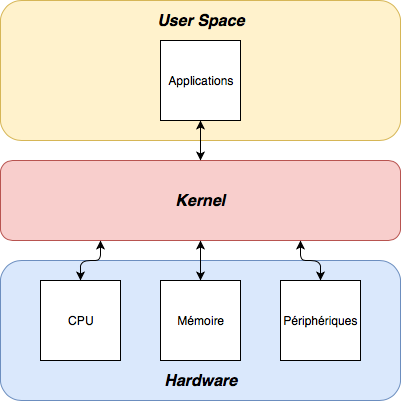
\includegraphics[scale=0.75]{images/kernel.png}
    \caption{Architecture du système d'exploitation}
    \label{os_arch}
\end{figure}

%%%%%%%%%%%%%%%%%%%%%%%%%%%%%%%%%%%%%%%%%%%%%%%%%%%%%%%%%%%%%%%%%%
%%%%%%%%%%%%%%%%%%%%%%%%%%%%%%%%%%%%%%%%%%%%%%%%%%%%%%%%%%%%%%%%%%

\subsection{Environnement de développement}
La machine utilisée pour le développement du projet est un MacBook Pro avec un
processeur Intel à 3 GHz. Il a quand même fallut utiliser une machine virtuelle
(VMware) utilisant Linux (Ubuntu 16.04.4 LTS) pour la compilation. Ce choix a été
fait car il existe beaucoup plus de documentation sur l'implémentation de systèmes
d'exploitation sur Linux que sur Mac. Bien que Mac \acrshort{os} soit un système
UNIX, les exécutables générés sur cet environnement n'ont pas le même format que
ceux générés sur Linux qui sont au format \acrshort{elf}. Ceci rend le développement
d'\acrshort{os} légèrement différent sur Mac \acrshort{os}. Linux est donc utilisé
pour la compilation et l'exécution du système d'exploitation. \\

Le code doit être compilé pour être exécutable sous une architecture \acrshort{IA-32}.
La compilation du code Rust est expliquée dans le chapitre \ref{rust_compil}. Certaines
parties du code du \textit{kernel} ont été écrites en assembleur car étant trop bas niveau
pour Rust. Nasm a été  utilisé pour compiler le code assembleur x86 en \acrshort{elf}
32 bits. Nasm produit des fichiers objets pouvant être liés à d'autres fichiers
objets (comme ceux générés par Rust) afin de créer un exécutable. Tout le mécanisme
de génération d'un \textit{kernel} exécutable est décrit en détail dans le chapitre
\ref{execution}. Pour ce projet, une machine virtuelle est utilisée pour démarrer
sur notre système d'exploitation. Cette machine virtuelle est QEMU. Elle peut
émuler plusieurs architectures dont l'architecture i386 qui nous intéresse ici.
QEMU peut démarrer un système d'exploitation depuis un fichier \acrshort{iso}
ou bien directement depuis un exécutable au format \acrshort{elf}. Dans notre
cas, un fichier \acrshort{iso} contenant le \textit{kernel} est généré.

\begin{figure}[!h]
    \centering
    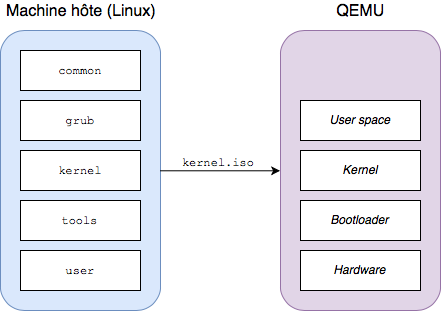
\includegraphics[scale=0.75]{images/global_arch.png}
    \caption{Architecture globale du projet}
    \label{os_arch}
\end{figure}

\newpage
%%%%%%%%%%%%%%%%%%%%%%%%%%%%%%%%%%%%%%%%%%%%%%%%%%%%%%%%%%%%%%%%%%
%%%%%%%%%%%%%%%%%%%%%%%%%%%%%%%%%%%%%%%%%%%%%%%%%%%%%%%%%%%%%%%%%%

\section{Langage Rust}

\newpage
%%%%%%%%%%%%%%%%%%%%%%%%%%%%%%%%%%%%%%%%%%%%%%%%%%%%%%%%%%%%%%%%%%
%%%%%%%%%%%%%%%%%%%%%%%%%%%%%%%%%%%%%%%%%%%%%%%%%%%%%%%%%%%%%%%%%%

\section{Exécution du \textit{kernel}}
%%%%%%%%%%%%%%%%%%%%%%%%%%%%%%%%%%%%%%%%%%%%%%%%%%%%%%%%%%%%%%%%%%
%%%%%%%%%%%%%%%%%%%%%%%%%%%%%%%%%%%%%%%%%%%%%%%%%%%%%%%%%%%%%%%%%%

\subsection{Compilation}
Quand on veut compiler un simple code C en utilisant \acrshort{gcc} par
exemple, le compilateur passe par plusieurs étapes. Le préprocesseur génère d'abord
un fichier C en fonction des directives de préprocesseur. Ce fichier C est ensuite
compilé en code assembleur qui est lui même compilé en code objet. Le \textit{linker}
permet ensuite de lier les différents fichiers objets et générer un exécutable.
Nous avons déjà eu un aperçu des différentes étapes de la compilation d'un \acrshort{os}
de type \textit{bare metal} dans la partie 3.2. A la différence de la compilation
d'un code C, nous avons d'un côté du code assembleur et de l'autre du code Rust.
Nasm et cargo permettent tous deux de générer des fichiers objets. Il n'y a donc
que la dernière étape à effectuer ce que \acrshort{gcc} permet de faire avec
la commande suivante.
\begin{minted}[tabsize=4]{shell}
gcc $(OBJS) -T $(LINKER) -static -m32 -ffreestanding -nostdlib -o $@ $(RUST)
\end{minted}
Ici, \mintinline{shell}{$(OBJS)} représente les fichiers objets générés par
\mintinline{rust}{nasm}, \mintinline{shell}{$(LINKER)} est un fichier permettant
de faire l'édition des liens et \mintinline{shell}{$(RUST)} représente les fichiers
objets générés par Rust.\cite{ref42}

%%%%%%%%%%%%%%%%%%%%%%%%%%%%%%%%%%%%%%%%%%%%%%%%%%%%%%%%%%%%%%%%%%
%%%%%%%%%%%%%%%%%%%%%%%%%%%%%%%%%%%%%%%%%%%%%%%%%%%%%%%%%%%%%%%%%%

\subsection{\textit{Linking}}
Nous avons vu dans la partie précédente que \acrshort{gcc} a besoin d'un fichier
pour faire l'édition des liens. Si ce fichier n'est pas donné, il en utilise un par
défaut. Le \textit{linker} permet de structurer le code par sections. Prenons
pour exemple le \textit{script} utilisé pour ce projet.

\begin{minted}[fontsize=\footnotesize,linenos,frame=single,tabsize=4]{c}
ENTRY(entrypoint)
SECTIONS {
  . = 1M;
  .boot ALIGN(4):
  {
    *(.multiboot)
  }
  .stack ALIGN(4):
  {
    *(.stack)
  }
  .text ALIGN(4K) :
  {
    *(.text*)
  }
  .rodata ALIGN(4K) :
  {
    *(.rodata*)
  }
  .data ALIGN(4K) :
  {
    *(.data*)
  }
  .bss ALIGN(4K) :
  {
    *(COMMON)
    *(.bss*)
  }
}
\end{minted}

L'appel à \mintinline{c}{ENTRY} permet de spécifier l'entrée du \textit{kernel}.
Pour un simple programme en C l'entrée serait le \textit{main}. Ici, ce sera
l'entrée de notre \textit{kernel} donc la première fonction exécutée au \textit{boot}.
\mintinline{text}{SECTION} va dire au linker où placer les parties du code. Par exemple, 
la section \mintinline{text}{.text} contiendra le code et la section \mintinline{text}{.data}
contiendra les variables initialisées \cite{ref42,ref9,ref10,ref11}. Voici donc la structure
du fichier \acrshort{elf} qui serait généré à l'aide de ce \textit{script}.

\begin{figure}[!h]
  \centering
  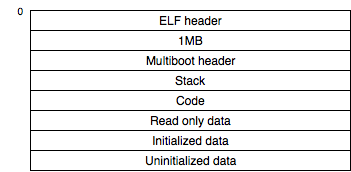
\includegraphics[scale=0.75]{images/elf_struct.png}
  \caption{Strucutre du fichier \acrshort{elf}}
\end{figure}

A noter que les sections commencent avec un \textit{offset} de 1MB. Nous avons eu
besoin de faire ça car les premiers 1MB dans un \acrshort{os} sont reservés \cite{ref42,ref13}.
La mémoire vidéo (\acrshort{vram}) se situe par exemple dans cette zone.

%%%%%%%%%%%%%%%%%%%%%%%%%%%%%%%%%%%%%%%%%%%%%%%%%%%%%%%%%%%%%%%%%%
%%%%%%%%%%%%%%%%%%%%%%%%%%%%%%%%%%%%%%%%%%%%%%%%%%%%%%%%%%%%%%%%%%

\subsection{\textit{Boot}}
\subsubsection{Principe général}
Quand un ordinateur est allumé, un signal est envoyé à la carte mère qui démarre
l'alimentation. Le processeur démarre alors en mode 16-bits. Le signal "Power Ok"
est envoyé au \acrshort{bios} qui est le \textit{firmware} du \acrshort{pc}
(localisé en mémoire flash de la carte mère). Le \acrshort{bios} initialise alors
la séquence POST (\textit{Power On Self Test}) qui vérifie que chaque périphérique
est alimenté et que la mémoire est ok puis initialise chaque périphérique et enfin
redonne la main au \acrshort{bios} qui continue le \textit{boot}. Le \acrshort{bios}
charge ensuite les 512 premiers bytes (\acrshort{mbr}) du premier disque qui doit
charger le \textit{kernel} en mémoire et l'exécuter. Pour résumer, le \textit{boot}
d'une machine à base de \acrshort{bios} se déroule de la manière ci-dessous.\cite{ref42}

\begin{figure}[!h]
  \centering
  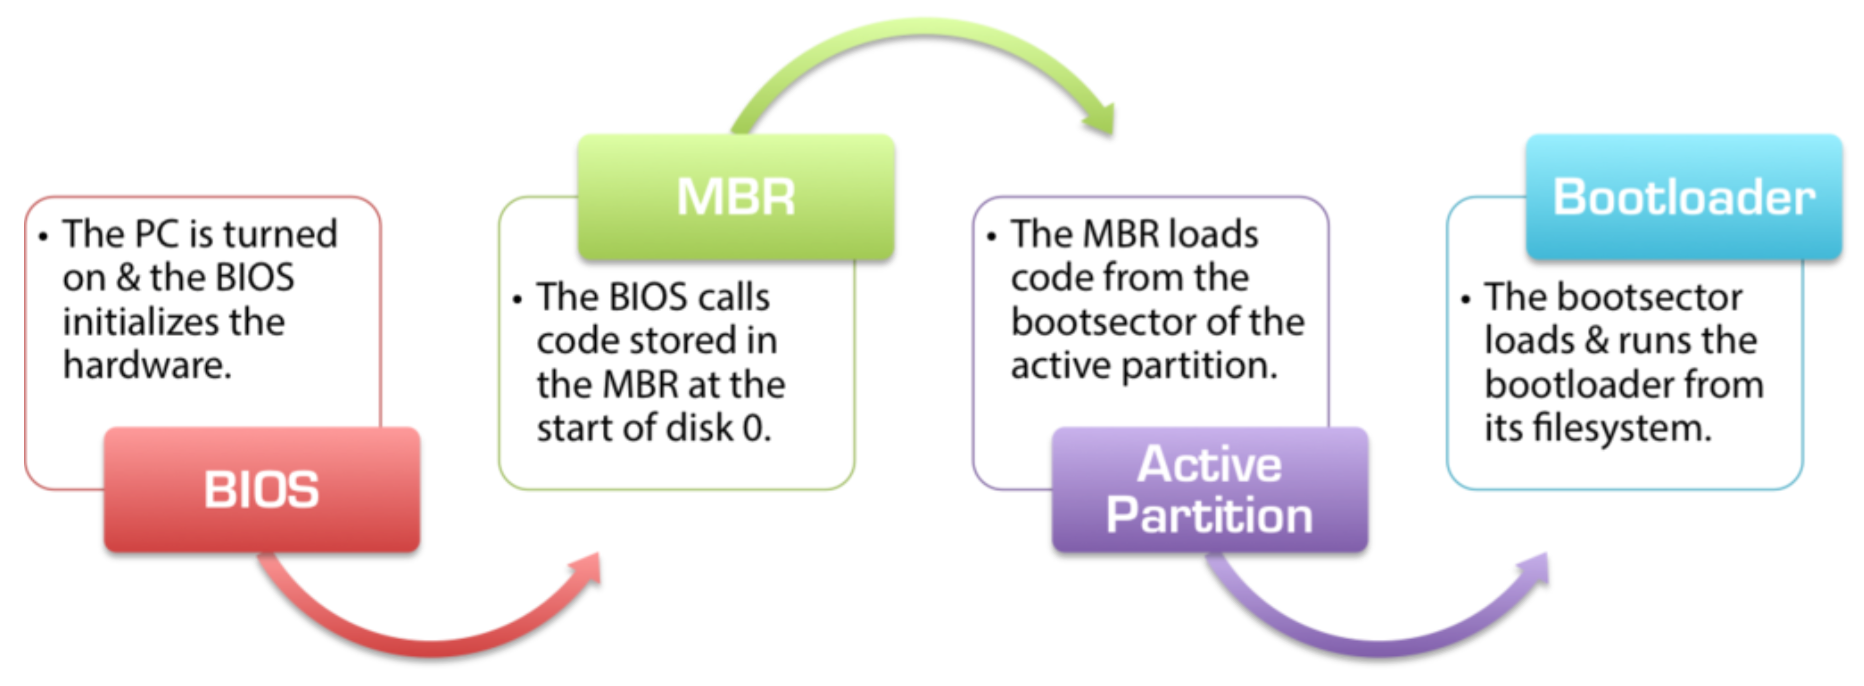
\includegraphics[scale=0.4]{images/bios_boot.png}
  \caption{\textit{Boot} d'une machine à base de \acrshort{bios}}
\end{figure}

%%%%%%%%%%%%%%%%%%%%%%%%%%%%%%%%%%%%%%%%%%%%%%%%%%%%%%%%%%%%%%%%%%

\subsubsection{\acrshort{grub}}
Le \acrshort{mbr} contient ce qui est appelé le \textit{bootloader}. Le \textit{bootloader}
est le morceau de code qui va charger le \textit{kernel} en mémoire et l'exécuter.
C'est ici qu'entre en scène \acrshort{grub}. \acrshort{grub} est un \textit{bootloader}
puissant et versatile permettant de charger n’importe quel type de système d’exploitation.
Son initialisation se fait par étapes.
\begin{itemize}[label=\textbullet]
	\item \textit{Stage} 1: Chargé en mémoire par le \acrshort{bios} depuis le
    \acrshort{mbr}, il contient le code pour charger le \textit{Stage} 1.5
	\item \textit{Stage} 1.5: Chargé en mémoire par le \textit{Stage} 1, il contient
    les drivers nécessaires à l'accès au système de fichiers par le \textit{Stage} 2
	\item \textit{Stage} 2: Chargé en mémoire par le \textit{Stage} 1.5, il affiche
    le menu de \acrshort{grub}. Il permet de sélectionner et charger un \acrshort{os}
\end{itemize}

\acrshort{grub} permet de charger n'importe quel type de système d'exploitation
grace au standard \textit{Multiboot}. Ce standard permet à tout \textit{bootloader}
de charger tout \acrshort{os} compatible \cite{ref42,ref12}.

\subsubsection{Image \acrshort{iso}}
Nous avons déjà pu voir que le \textit{boot} du \textit{kernel} se faisait à partie
d'une image \acrshort{iso} dans la partie 3.2.4. Pour qu'une image \acrshort{iso}
soit \textit{bootable}, il est nécessaire que \acrshort{grub} soit installé dans
les huit premiers KB du disque. Prenons l'arborescence suivante :

\begin{minted}[tabsize=4]{shell}
isofiles
└── boot
    └── grub
\end{minted}

Les fichiers \mintinline{text}{kernel.elf} (kernel sur lequel nous voulons
\textit{booter}), \mintinline{text}{menu.lst} (fichier de configuration de \acrshort{grub})
et \mintinline{text}{stage2_eltorito} doivent être copiés de manière à obtenir
l'arborescence suivante :

\begin{minted}[tabsize=4]{text}
isofiles
└── boot
    ├── grub
    │   ├── menu.lst
    │   └── stage2_eltorito
    └── kernel.elf
\end{minted}

Pour finir, il faut exécuter la commande :
\begin{minted}[tabsize=4]{shell}
genisoimage -R -b boot/grub/stage2_eltorito -input-charset utf8 -no-emul-boot \
-boot-info-table -o os.iso isofiles
\end{minted}
Cette commande génerera une image \acrshort{iso} \textit{bootable} nommée \mintinline{text}{os.iso}\cite{ref42}.

\newpage
%%%%%%%%%%%%%%%%%%%%%%%%%%%%%%%%%%%%%%%%%%%%%%%%%%%%%%%%%%%%%%%%%%
%%%%%%%%%%%%%%%%%%%%%%%%%%%%%%%%%%%%%%%%%%%%%%%%%%%%%%%%%%%%%%%%%%

\section{Gestion mémoire}
%%%%%%%%%%%%%%%%%%%%%%%%%%%%%%%%%%%%%%%%%%%%%%%%%%%%%%%%%%%%%%%%%%
%%%%%%%%%%%%%%%%%%%%%%%%%%%%%%%%%%%%%%%%%%%%%%%%%%%%%%%%%%%%%%%%%%

\subsection{Introduction}
Le système d'exploitation développé est exécuté sur une architecture \acrshort{IA-32}
(Intel 32-bits) aussi appelée i386. La mémoire est donc adressée sur 32 bits.
$2^{32}=4Go$, on peut en déduire que la taille totale de la mémoire adressable est
de 4Go dans notre système d'exploitation. Avoir un espace adressable de 4Go ne veut
pas forcément dire que la mémoire physique (\acrshort{ram}) est de 4Go aussi. En
réalité, la taille de la \acrshort{ram} dépend du \textit{hardware}. Dans notre
cas le matériel est émulé par QEMU. La taille de la mémoire physique de notre \acrshort{os}
dépend de la configuration de l'émulateur. Ces 4Go sont donc virtuels. Lorsqu'une
tache est exécutée, elle est chargée en mémoire et est définie par la paire base
et limite. La base est son adresse physique dans la \acrshort{ram} et la limite
est sa taille. La figure \ref{ex_base_limit} donne un exemple d'adressage de plusieurs
processus \cite{ref42}.

\begin{figure}[!h]
  \centering
  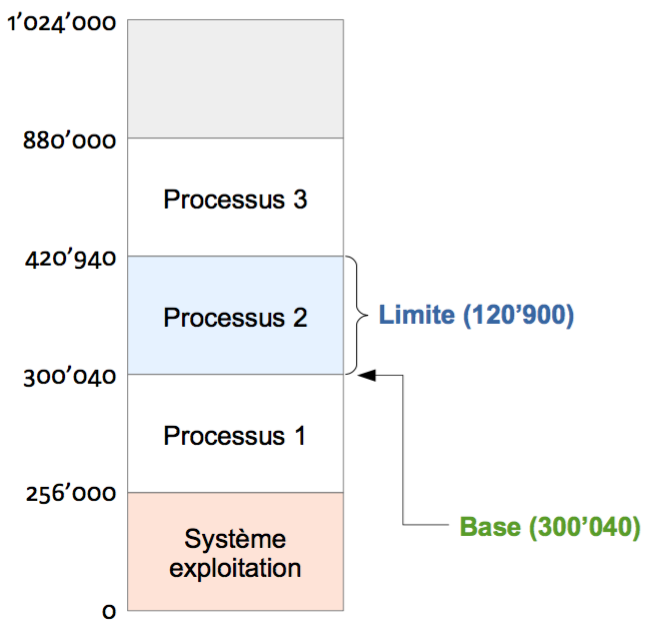
\includegraphics[scale=0.6]{images/ex_base_limit.png}
  \caption{Exemple d'adressage mémoire}
  \label{ex_base_limit}
\end{figure}

Une tache possède son propre espace d'adressage dit virtuel. Pour le processus 2
de la figure \ref{ex_base_limit}, l'adresse $0$ est en fait à l'adresse physique
$300040$. Il y a donc besoin de translater l'adresse virtuelle en adresse physique.
C'est là qu'entre en jeu le \acrshort{mmu} (Memory Mangement Unit). Le \acrshort{mmu}
est un dispositif matériel permettant de faire cette translation d'adresses. A chaque
référencement mémoire, il va convertir l'adresse virtuelle en adresse physique et
regarder si elle ne dépasse pas la limite du processus. Le \acrshort{mmu} permet donc
aussi de protéger la mémoire car il va empêcher toute référence à une zone extérieure
au processus (voir figure \ref{mmu}) \cite{ref42}.

\begin{figure}[!h]
  \centering
  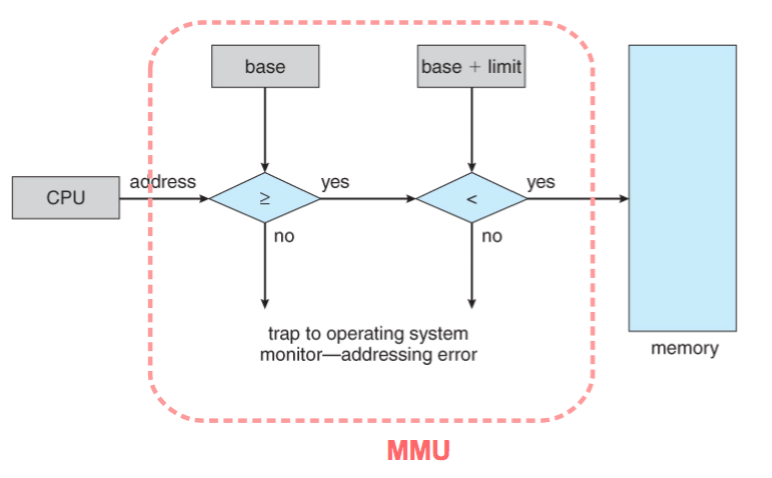
\includegraphics[scale=0.4]{images/mmu.png}
  \caption{Protection mémoire avec un \acrshort{mmu}}
  \label{mmu}
\end{figure}

Pour convertir une adresse virtuelle en adresse physique, le \acrshort{mmu} passe
par plusieurs étapes. Quand le \textit{kernel} veut lire une donnée dans la mémoire,
l'adresse de cette donnée est appelée adresse logique. Le \acrshort{mmu} va commencer
par convertir cette adresse en adresse linéaire. Une deuxième conversion est ensuite
effectuée afin d'obtenir une adresse physique. Le \acrshort{mmu} peut alors renvoyer
la bonne donnée au \textit{kernel}. Toutes ces étapes ne sont pas automatiques,
le \acrshort{mmu} utilise différentes techniques ayant besoin de certaines structures
implémentées par le \textit{kernel}. Ces techniques sont la segmentation et la
pagination.

\begin{figure}[!h]
  \centering
  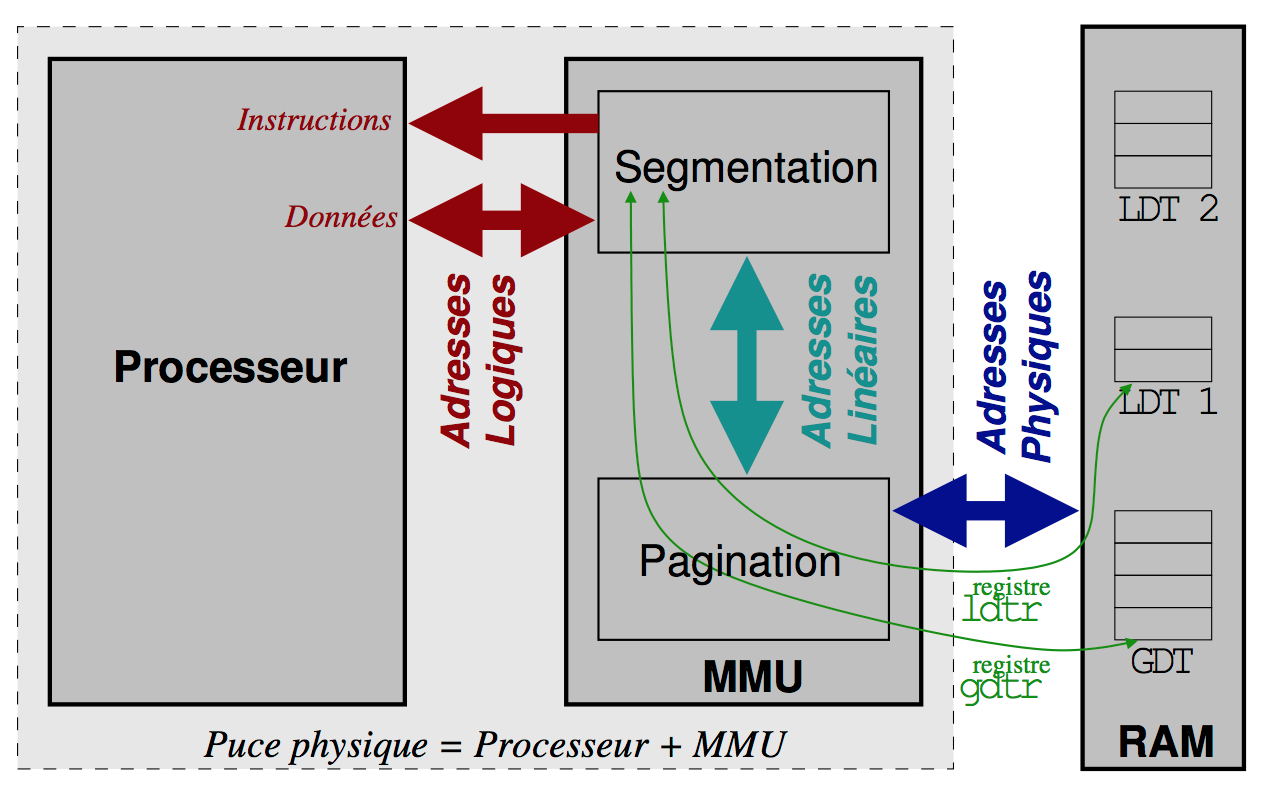
\includegraphics[scale=0.5]{images/addr_translation.png}
  \caption{Translation d'adresse}
  \label{addr_translation}
\end{figure}

La segmentation est une technique permettant de découper la mémoire en segments
de mémoire logique. Une adresse logique est convertie par le \acrshort{mmu} en
adresse linéaire en utilisant une table de descripteurs globale (\acrshort{gdt})
ou locale (\acrshort{ldt}). Si la pagination est activée, l'adresse linéaire est
convertie en adresse physique. Toute cette mécanique est décrite dans la figure
\ref{addr_translation}. A noter que la pagination n'est pas obligatoire et un
\acrshort{os} pourrait s'en passer contrairement à la segmentation qui est
indispensable en mode protégé (32-bits) \cite{ref17}.

%%%%%%%%%%%%%%%%%%%%%%%%%%%%%%%%%%%%%%%%%%%%%%%%%%%%%%%%%%%%%%%%%%
%%%%%%%%%%%%%%%%%%%%%%%%%%%%%%%%%%%%%%%%%%%%%%%%%%%%%%%%%%%%%%%%%%

\subsection{Segmentation}
\subsubsection{Principe général}
Comme expliqué précedemment, la segmentation est un mécanisme divisant l'espace
d'adressage du processeur en espaces d'adressage plus petits appelés des
segments. Un segment peut être utilisé pour contenir le code, les données ou la
pile d'un processus étant exécuté par le processeur. Un segment peut aussi être
utilisé pour contenir des structures de données tel qu'une \acrshort{ldt} ou
un \acrshort{tss} (structure contenant des informations à propos d'une tâche).
Les segments d'un système d'exploitation sont contenus dans l'espace d'adressage
linéaire. Pour lire l'octet d'un segment se trouvant dans l'espace d'adressage
linéaire, le \acrshort{mmu} utilise une adresse logique. L'adresse logique est
composée d'un sélecteur de segment et d'un \textit{offset}. Le sélecteur permet
de trouver le bon segment dans la mémoire linéaire et l'\textit{offset} permet
de trouver l'octet dans ce segment. Dans le cas où la segmentation est utilisée
seule (sans pagination), la mémoire linéaire est \textit{mappée} directement dans
la mémoire physique \cite{ref66}. \\

\begin{figure}[!h]
  \centering
  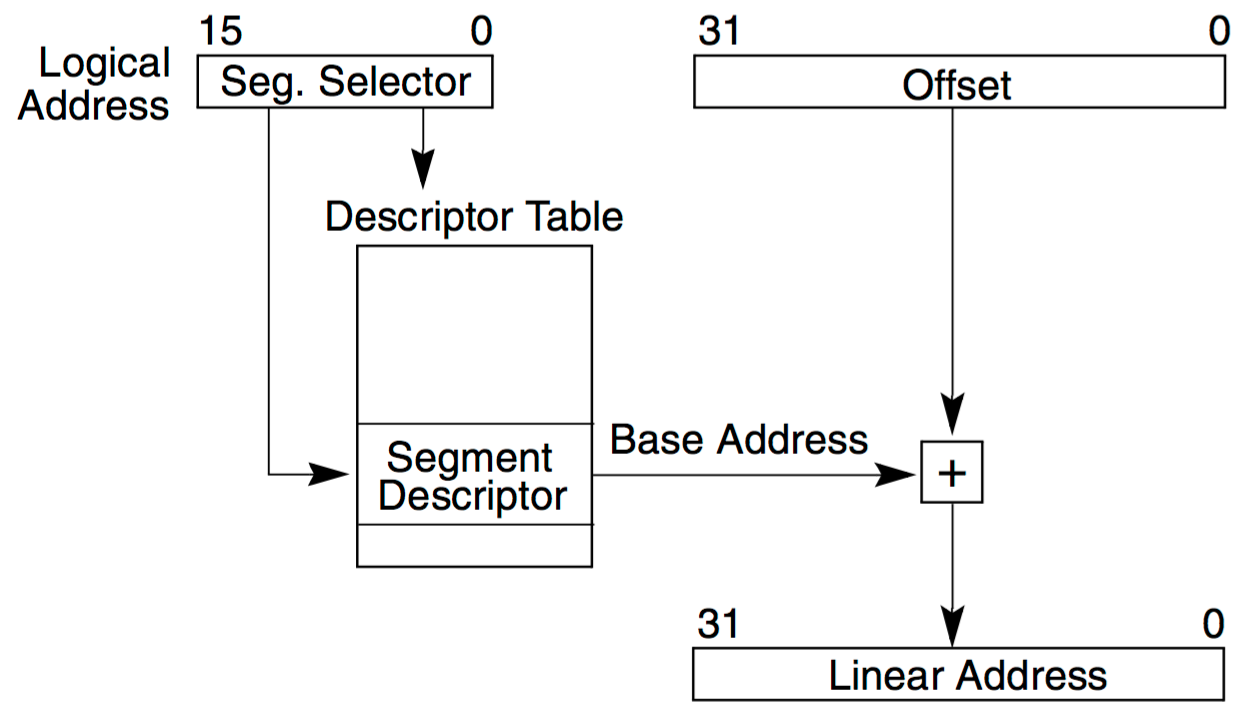
\includegraphics[scale=0.45]{images/logic_addr_conv.png}
  \caption{Conversion d'une adresse logique en adresse linéaire}
  \label{logic_addr_conv}
\end{figure}

La figure \ref{logic_addr_conv} résume bien la conversion d'adresse logique en
en adresse linéaire. On peut remarquer de plus que le sélecteur de segment passe
par une table de descripteurs (\acrshort{gdt} ou \acrshort{ldt}) afin de trouver
le bon segment dans la mémoire linéaire. En effet, Un sélecteur a une taille de
16 bits et contient l'index d'un descripteur dans une table, un bit indiquant si
le descripteur est dans la \acrshort{gdt} ou dans une \acrshort{ldt} et enfin son
niveau de privilège allant de 0 à 3 (figure \ref{seg_sel}) \cite{ref42}.

\begin{figure}[!h]
  \centering
  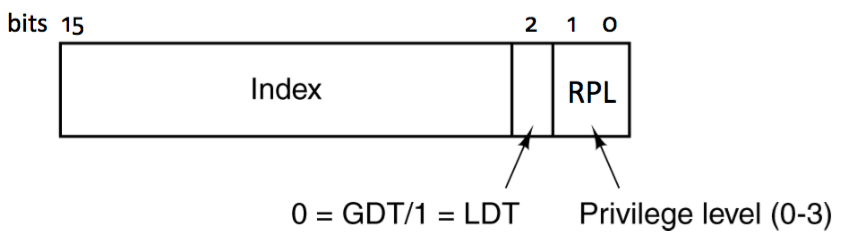
\includegraphics[scale=0.6]{images/seg_sel.png}
  \caption{Structure d'un sélecteur de segment}
  \label{seg_sel}
\end{figure}

La gestion de la segmentation par le \acrshort{cpu} se fait à l'aide de registres
spéciaux nommés registres de segment. Ces registres sont au nombre de six et ont
chacun une taille de 16 bits (même taille qu'un sélecteur de segment) \cite{ref42,ref18}.

\begin{center}
	\scalebox{.8}{
		\begin{tabular}{| C{5cm} | C{5cm} | }
			\hline
			Registre & Segment \\ \hline
			CS & \textit{Code Segment} \\ \hline
			DS & \textit{Data Segment} \\ \hline
			SS & \textit{Stack Segment} \\ \hline
			ES & \textit{Extra Segment} \\ \hline
			FS & \multirow{2}{*}{\textit{General Purpose Segments}} \\
            GS & \\ \hline
		\end{tabular}
	}
\end{center}

En mode protégé (32-bits), ces registres doivent pointer sur des descripteurs
de segment de la \acrshort{gdt}. Au minimum les trois premiers registres décrits
doivent être utilisé en mode protégé (CS, DS, et SS). Les opérations adressant
le code (décodage des instructons en mémoire, sauts, etc...) référencent le descripteur
de segment sur lequel pointe le registre CS. Les opérations adressant les données
(adressage de variables ou d'adresses mémoires) référencent le descripteur de segment
sur lequel pointe le registre DS. Les opérations adressant la pile (\mintinline{text}{push}
et \mintinline{text}{pop}) référencent le descripteur de segment sur lequel pointe
le registre SS. Ces registres pointent sur des descripteurs de segments par l'intermédiaire
de sélecteurs de segment. \\

\subsubsection{\acrshort{gdt} et \acrshort{ldt}}
\label{gdt_ldt}
Nous avons pu voir que pour translater une adresse logique, des sélecteurs de
segment sont utilisés. Ces sélecteurs pointent sur des entrées dans des tables
de descripteurs. La \acrshort{gdt} et la \acrshort{ldt} sont deux types de table 
de descripteurs différents. La \acrshort{gdt} est unique il ne peut y en avoir
qu'une seule dans le système. Elle contient toutes les données utilisables en mode
superviseur (\textit{ring} 0 ou niveau de privilège 0). Une \acrshort{ldt} est
contenue dans la \acrshort{gdt}. Elle peut être utilisée pour contenir le code
et les données d'une tâche utilisateur par exemple. Dans le cas où plusieurs tâches
sont exécutées en même temps, une \acrshort{ldt} peut être créée par tâche ce qui
permet en plus d'isoler le code de chaque processus. Une table de descipteurs
est composée, comme son nom l'indique, de descripteurs. Chaque descripteur décrit
une zone mémoire qui est défini par sa base (son adresse physique), sa limite (sa taille)
et un niveau de privilèges (allant de 0 à 3, le niveau 0 ayant le plus de privilèges
et le niveau 3 le moins). Ci dessous, la figure \ref{gdt} montre un exemple d'une
\acrshort{gdt} \cite{ref42}. Etant donné que les descripteurs de la \acrshort{gdt}
ont la même structure que les descripteurs de la \acrshort{ldt} nous allons nous
concentrer sur la \acrshort{gdt}. De plus, aucune \acrshort{ldt} n'est utilisé dans
la version actuelle de l'\acrshort{os}. \\

\begin{figure}[!h]
  \centering
  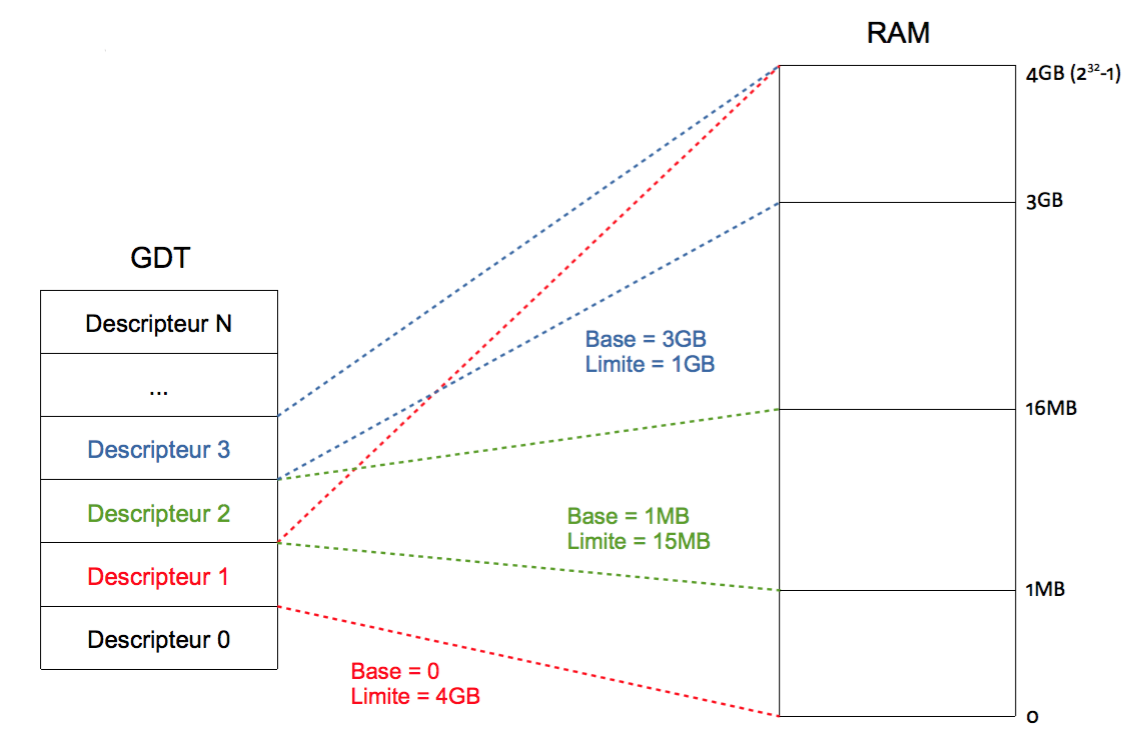
\includegraphics[scale=0.75]{images/gdt.png}
  \caption{Exemple d'une \acrshort{gdt}}
  \label{gdt}
\end{figure}

La \acrshort{gdt} est contenue en mémoire. Cette dernière doit être initialisée
par le \textit{kernel} avant d'être chargée et utilisée par le \acrshort{mmu}.
Pour initialiser la \acrshort{gdt} il faut construire ses entrées. Chaque entrée
(ou descripteur) de la table de descripteurs est sur 64 bit et décrit une zone
mémoire. L'adresse de cette zone mémoire est sur 32 bits et sa taille est sur 20
bits. Les bits restant sont des bits de contrôle pour l'accès aux données par
exemple (niveau de privilèfes, droit d'écriture/lecture, ...). Voir la figure
\ref{gdt_entry} pour plus de détails \cite{ref42,ref14}. \\

\begin{figure}[!h]
  \centering
  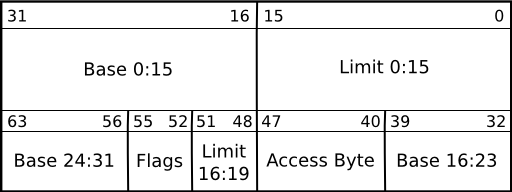
\includegraphics[scale=0.75]{images/gdt_entry.png}
  \caption{Structure d'une entrée dans la \acrshort{gdt}}
  \label{gdt_entry}
\end{figure}

L'\acrshort{os} développé a un adressage segmenté de type \textit{flat}, c'est-à-dire
que toute la mémoire est accédée de manière linéaire. Ce modèle de segmentation
est le plus simple car il permet d'ignorer le mécanisme de segmentation car
l'intégralité de la zone mémoire devient disponible. Dans un modèle de type \textit{flat},
les segments de code et de données se chevauchent sur l'intégralité de la mémoire
disponible. Ceci se fait en initialisant trois descripteurs dans la \acrshort{gdt}.
Un descripteur nul à l'index 0 (obligatoire dans touts les modèles de segmentation),
un segment de code couvrant toute la mémoire et un segment de données couvrant
aussi toute la mémoire. Les segments de code et de données adressent ainsi les mêmes
zones mémoire. On verra par la suite que d'autres entrées ont été aujoutées à la
\acrshort{gdt} pour la gestion des tâches. \\

\begin{figure}[!h]
  \centering
  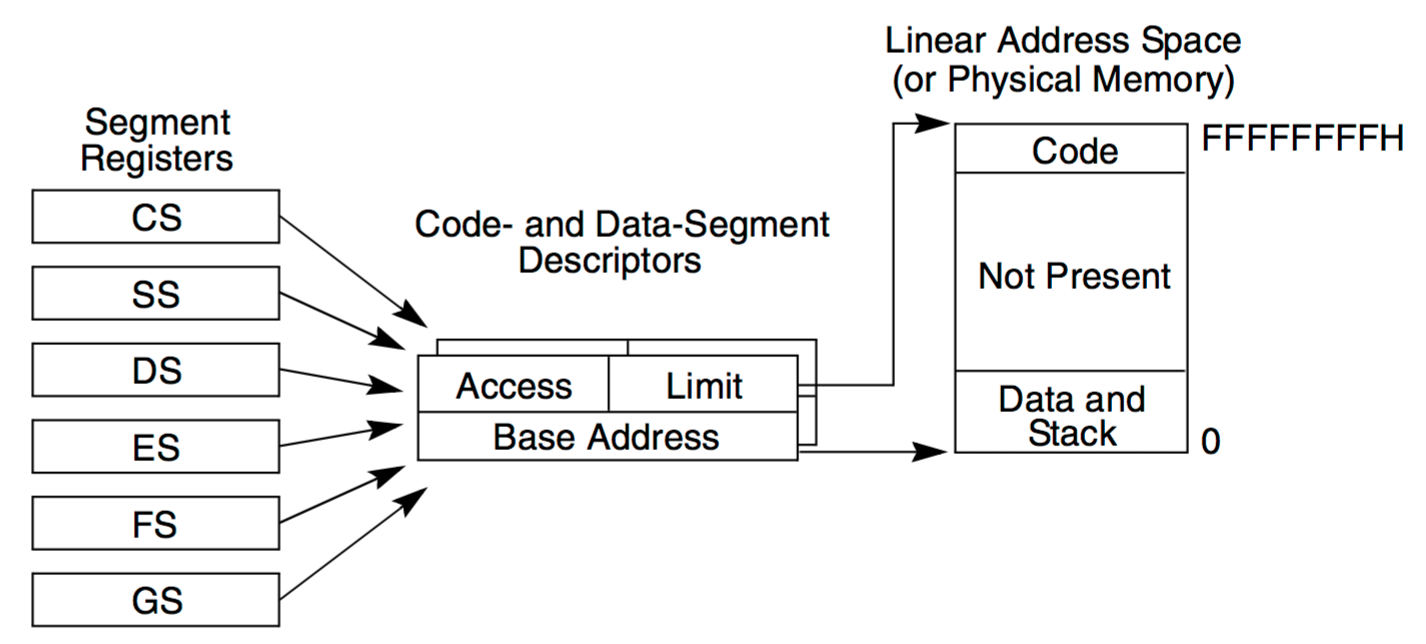
\includegraphics[scale=0.6]{images/flat.png}
  \caption{Modèle de segmentation de type \textit{flat}}
  \label{flat}
\end{figure}

Pour obtenir un  segment sur toute la mémoire disponible, il faut mettre le bit
de granularité à 1 pour avoir une limite en blocs de 4Ko. Ensuite, la limite doit
être mise à la valeur 0xFFFFF ce qui donne une limite réele de 0x100000 $\times$
0x1000 soit 4Go. Le niveau de privilège doit être laissé à 0 (\textit{ring} 0)
si on veut créer un segment pour le \textit{kernel} ou bien être mis à 3 (\textit{ring}
3) si on veut créer un segment pour le mode utilisateur. Ci-dessous un exemple de
code permettant de construire un segment de code et un segment de données. \\

\begin{minted}[fontsize=\footnotesize,tabsize=4,frame=single]{rust}
fn new(base: u32, limit: u32, type: u8, s: u8, d: u8, g: u8, dpl: u8) -> GdtEntry;

pub fn make_code_segment(base: u32, limit: u32, dpl: u8) -> GdtEntry {
    GdtEntry::new(base, limit, 0xB, 0x1, 0x1, 0x1, dpl)
}

pub fn make_data_segment(base: u32, limit: u32, dpl: u8) -> GdtEntry {
    GdtEntry::new(base, limit, 0x3, 0x1, 0x1, 0x1, dpl)
}
\end{minted}

Ici, \mintinline{rust}{new} est le prototype d'une méthode pour une structure 64
bits représentant une entrée dans la \acrshort{gdt}. le bit \mintinline{rust}{s}
est mis à 1 car on construit des segments de code et de données \cite{ref66}.
Le bit \mintinline{rust}{d} est mis à 1 car on veut un segment de 32 bits. Le bit
\mintinline{rust}{g} est mis à 1 pour avoir une granularité de 4Ko. L'octet 0xB
correspond au type $CODE\_EXEC\_READ$ et 0x3 correspond au type $DATA\_READ\_WRITE$
\cite{ref42}. Une fois la \acrshort{gdt} construite, il faut dans un premier temps
utiliser l'instruction \mintinline{text}{lgdt} pour la charger dans le registre
GDTR. Ce registre est utilisé par le processeur pour faire le lien entre le \acrshort{mmu}
et la \acrshort{gdt} créée \cite{ref66}. L'adresse du descripteur de la \acrshort{gdt}
doit donc être donnée en argument à l'instruction \mintinline{text}{lgdt}. Le
descripteur de \acrshort{gdt} est défini par la structure 48-bits décrite dans
la figure \ref{gdt_descriptor} \cite{ref14}.

\begin{figure}[!h]
  \centering
  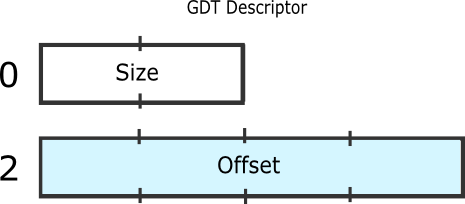
\includegraphics[scale=0.5]{images/gdt_descriptor.png}
  \caption{Descripteur de \acrshort{gdt}}
  \label{gdt_descriptor}
\end{figure}

Dans un descripteur de \acrshort{gdt} \textit{Size} est la limite sur 16 bits
(c'est à dire la taille de la \acrshort{gdt} - 1) et \textit{Offset} est l'adresse
physique de la \acrshort{gdt} sur 32 bits. Dans le cas de notre \acrshort{os},
la \acrshort{gdt} est déclarée statiquement dans le \textit{kernel}. L'adresse
de cette variable statique est utilisée pour construire un descripteur qui sera
chargé dans le registre GTDR. Après avoir chargé la \acrshort{gdt} avec l'instruction
\mintinline{text}{lgdt}, il faut faire pointer les registres de segment sur les
segments de la table de descripteurs à l'aide de sélecteurs. Pour rappel, un sélecteur
est sur 16 bits et contient l'index d'un segment dans la \acrshort{gdt} précedemment
chargée. Pour récupérer l'index d'un segment dans la \acrshort{gdt} à partir de
l'index de son descripteur, il faut faire un décallage à gauche de 3 bits
(voir figure \ref{seg_sel}). Prennons un descripteur se situant à l'index 2 de
la \acrshort{gdt}. Si on veut initialiser le segment de code (registre CS) avec
ce descripteur, il faut mettre la valeur 16 dans le registre CS ($2 << 3 = 16$).
Dans le cas où on veut définir ce segment avec un autre niveau de privilèges
ou bien pour une \acrshort{ldt}, il suffit de mettre les bons bits à 1 après avoir
fait le décallage.

\newpage
%%%%%%%%%%%%%%%%%%%%%%%%%%%%%%%%%%%%%%%%%%%%%%%%%%%%%%%%%%%%%%%%%%
%%%%%%%%%%%%%%%%%%%%%%%%%%%%%%%%%%%%%%%%%%%%%%%%%%%%%%%%%%%%%%%%%%

\subsection{Pagination}
\subsubsection{Principe général}
La pagination est une autres technique de gestion de mémoire qui diffère de la
segmentation. Alors que la segmentation permet d'allouer des morceaux de mémoire
de taille variable, la pagination divise la mémoire en blocs de taille fixe appelés
pages (de 4Ko, 2Mo ou 4Mo). De plus, la segmentation est obligatoire dans une
architecture i386 alors que la pagination ne l'est pas \cite{ref16}. Quand une tâche
fait référence à une adresse logique en mémoire, cette adresse est convertie en
adresse linéaire grace au mécanisme de segmentation et c'est le mécanisme de
pagination qui permet de translater cette adresse linéaire en adresse physique
(comme vu précedemment dans la partie sur la segmentation). Quand la
pagination est activée, l'adresse linéaire est divisée en deux parties lorsque
des pages de 4Mo sont utilisées et en trois parties lorsque des pages de 4Ko
sont utilisées. Le \textit{kernel} développé utilise des pages de 4Ko, une adresse
linéaire est donc sous la forme suivante :

\begin{itemize}[label=\textbullet]
	\item 10 bits pour le \textit{directory index}
	\item 10 bits pour le \textit{page index}
    \item 12 bits pour l'\textit{offset}
\end{itemize}

On dit que cette pagination est une pagination à trois niveaux. En général, une
pagination à trois niveaux est utilisée mais il peut exister des systèmes utilisant
plus ou moins de niveaux. Le système d'exploitation doit créer un répertoire de pages
(\textit{Page Directory}) et au moins une table des pages (\textit{Page Table}) pour
chaque tâche. Les répertoires et les tables des pages ont la taille d'une page et sont
composés d'entrées sur 32 bits (4 octets). Une entrée dans un répertoire permet
d'adresser une table de pages et une entrée dans une table permet d'adresser une page.
Dans notre cas, un répertoire permet donc d'adresser 1024 tables et une table
1024 pages ce qui permet bien d'adresser au total 4Go ($1024 \times 1024 \times 4096$).
Une entrée est sur 32 bits mais seulement les 20 bits de poids fort sont utilisés
pour l'adressage car les adresses sont alignées avec 4096 ce qui laisse les 12 bits
de poids faible pour la configuration \cite{ref21}.

\begin{figure}[!h]
  \centering
  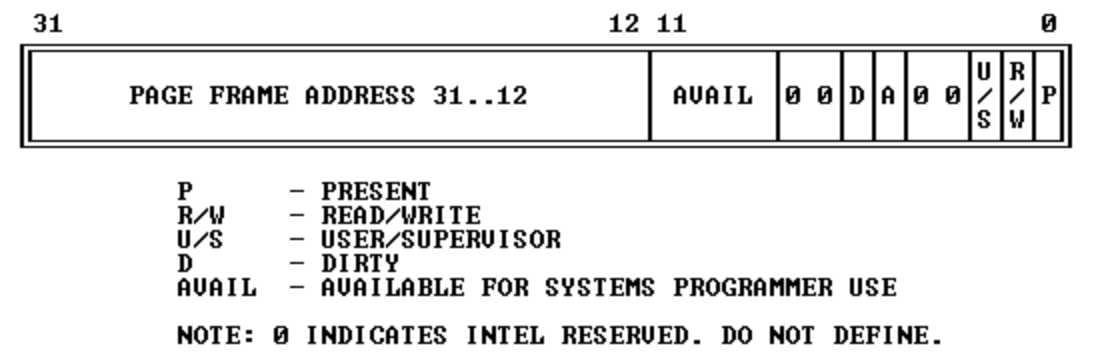
\includegraphics[scale=0.6]{images/page_entry.png}
  \caption{Structure d'une \textit{Page Entry}}
  \label{page_entry}
\end{figure}

Quand une adresse linéaire est lue, le \textit{directory index} permet
de lire la bonne entrée dans le \textit{Page Directory}. Il faut ensuite utiliser
le \textit{page index} pour récupérer la bonne entrée dans la table des pages.
De la même manière que l'entrée dans le répertoire de pages pointait sur une table
des pages, l'entrée dans une table des pages pointe sur une \textit{Page Frame}.
Cette page contient finalement la donnée pointée par l'adresse linéaire, il faut
utiliser l'\textit{offset} pour trouver cette donnée dans la page. La figure \ref{paging3}
résume bien ce mécanisme \cite{ref66}. A noter que le \textit{Page Directory} est
pointé par le registre CR3. A chaque fois qu'un changement de tâche a lieu, le
registre CR3 doit être mis à jour avec le \textit{Page Directory} de la nouvelle
tâche \cite{ref15}.

\begin{figure}[!h]
  \centering
  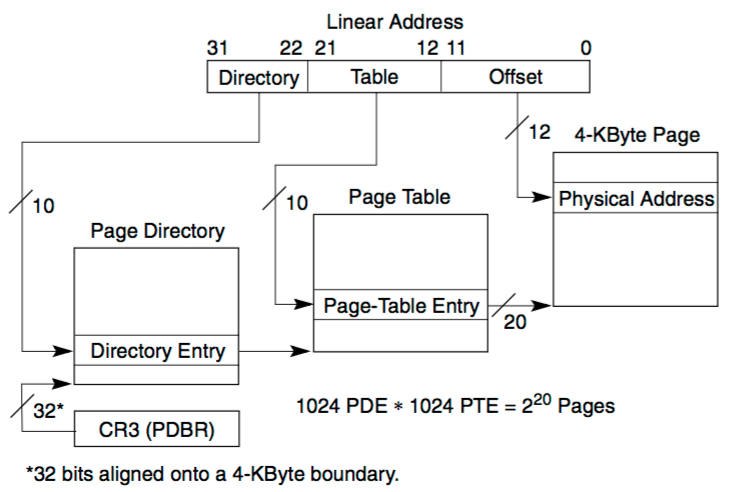
\includegraphics[scale=0.85]{images/paging3.png}
  \caption{Exemple de pagination à 3 niveaux}
  \label{paging3}
\end{figure}

%%%%%%%%%%%%%%%%%%%%%%%%%%%%%%%%%%%%%%%%%%%%%%%%%%%%%%%%%%%%%%%%%%

\subsubsection{Activation de la pagination}
\label{activate_paging}
Pour initialiser la pagination sur architecture x86, il faut d'abord construire
un répertoire de pages valide contenant les entrées vers les pages du \textit{kernel}.
Il est obligatoire de commencer par cela car si la pagination est activée et que
le \textit{kernel} n'est pas \textit{mappé} dans le répertoire chargé, une exception
sera levée (\textit{Page Fault}). Par soucis de simplicité pour la suite du développement
de l'\acrshort{os}, le \textit{kernel} va être déplacé au dernier Go de la \acrshort{ram}.
Grace à la pagination, ceci peut se faire assez simplement, il suffit de compléter
le répertoire de pages ainsi que ses tables de pages correctement. Pour rappel,
le \textit{kernel} commence à l'adresse 0x100000 (1Mo) mais il faut aussi rendre
accessible le premier Mo de \acrshort{ram}. Il faut donc déplacer les adresses physiques
allant de 0x0 à la fin du kernel (qui n'est pas fixe). Dans un premier temps, le
\textit{linker} doit être modifié de cette manière :

\begin{minted}[fontsize=\footnotesize,linenos,frame=single,tabsize=4]{c}
SECTIONS {
    /* Low memory Kernel */
    . = 0x00100000;
    .boot ALIGN(4) :        { *(.multiboot) }
    .low_text ALIGN (4K) :  { *(.low_text) }
    .low_data ALIGN (4K) :  { *(.low_data) }
    .low_bss ALIGN (4K) :   { *(.low_bss) }
    /* Higher-half Kernel */
    . += 0xC0000000;
    .stack ALIGN(4) : AT(ADDR(.stack) - 0xC0000000)     { *(.stack) }
    .text ALIGN(4K) : AT(ADDR(.text) - 0xC0000000)      { *(.text*) }
    .rodata ALIGN(4K) : AT(ADDR(.rodata) - 0xC0000000)  { *(.rodata*) }
    .data ALIGN(4K) : AT(ADDR(.data) - 0xC0000000)      { *(.data*) }
    .bss ALIGN(4K) : AT(ADDR(.bss) - 0xC0000000)        { *(COMMON) *(.bss*) }
}
\end{minted}

Ici, le \textit{kernel} est divisé en deux parties. La première est celle qui va
être appelée au démarrage du système et qui va initialiser la pagination. Une fois
la pagination active, le \textit{kernel} va continuer son exécution dans la deuxième
partie qui est située dans le dernier Go de \acrshort{ram}. Nous sommes obligés de
démarrer le \textit{kernel} au début de la mémoire physique car toutes les adresses
sont virtuelles. En réalité, le \textit{kernel} dispose de beaucoup moins (variable
selon la configuration de l'émulateur, ici QEMU). Il n'existe donc pas d'adresse
physique située à 3Go dans la mémoire physique du \textit{kernel} et il est donc
impossible de démarrer le système à cette adresse. Regardons plus en détail de quelle
manière la première partie du \textit{kernel} initialise la pagination. Comme dit
précedemment, un répertoire de pages initial doit être construit. Etant donné que
nous allons exécuter du code dans le premier Go et aussi dans le dernier, le \textit{kernel}
doit être \textit{mappé} dans ces deux zones mémoire en même temps. La première
partie va être adressée linéairement, ce qui veut dire que l'adresse physique
0x0 correspondra à l'adresse virtuelle 0x0 et ainsi de suite jusqu'à la fin du
\textit{kernel}. Cet adressage donne le répertoire de pages shématisé dans la figure
\ref{low_kern_pd}.

\begin{figure}[!h]
  \centering
  \includegraphics[scale=0.65]{images/low_kern_pd.png}
  \caption{Répertoire de pages adressant le \textit{kernel} au début de la \acrshort{ram}}
  \label{low_kern_pd}
\end{figure}

On peut voir ici que la première entrée du répertoire de pages pointe sur une
table de pages adressant le début de la \acrshort{ram}. Chaque entrée est incrémentée
de 4096 (0x1000 en hexadécimal) car une page fait 4096 octets. De plus, les deux
premiers bits de poids faible de chaque page sont à 1 pour indiquer que la page est
active et que l'on peut écrire et lire dedans (voir figure \ref{page_entry}). L'entrée
dans le répertoire de page correspondant au dernier Go (soit 0xC0000000 en hexadécimal)
doit pointer sur une table des pages identique. Pour trouver une entrée dans le
répertoire de pages depuis une adresse il faut faire un décallage à droite de 22
bits sur cette adresse (ce qui est équivalent à diviser par 4096, soit la taille
d'une page, puis de nouveau diviser par 1024, soit le nombre de pages adressées par
une table). Ici, 0xC0000000 $>>$ 22 = 0x300 (768 en décimal). Il faut donc faire
pointer l'entrée 768 du répertoire de pages à une table des pages identique à
celle pointée par l'entrée 0 ce qui donne finalement le répertoire suivant.

\begin{figure}[!h]
  \centering
  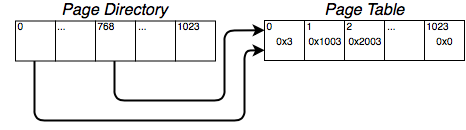
\includegraphics[scale=0.65]{images/high_kern_pd.png}
  \caption{Répertoire de pages adressant le \textit{kernel} à la fin de la \acrshort{ram}}
  \label{high_kern_pd}
\end{figure}

Une fois le répertoire de pages initialisé de cette manière, il ne reste plus
qu'à faire pointer le registre CR3 dessus et activer la pagination en mettant
le bit 31 du registre CR0 à 1. Le code peut ensuite sauter à la partie haute de
la \acrshort{ram} où nous avons déplacé le \textit{kernel}. A partir de là,
tout le code qui sera exécuté sera dans le dernier Go de \acrshort{ram}, il n'y
a donc plus besoin de faire pointer la première entrée du répertoire de pages
sur le table des pages du \textit{kernel} ce qui peut être fait en écrivant 0
dans cette entrée. Le code rust peut finalement être appelé avec la pagination
active.

%%%%%%%%%%%%%%%%%%%%%%%%%%%%%%%%%%%%%%%%%%%%%%%%%%%%%%%%%%%%%%%%%%

\subsection{Allocation dynamique en mode \textit{kernel}}
Le dernier élément de gestion mémoire implémenté dans RustOS est l'allocation de
mémoire dynamique. L'allocation dynamique consiste à réserver des blocs de mémoire
pendant l'exécution du \textit{kernel} ou bien d'un programme utilisateur. Jusqu'à
maintenant, toutes les structures utilisées était déclarées statiquement se retrouvant
donc dans la zone mémoire du \textit{kernel}, plus précisément dans le segment
bss (voir \ref{linking}). Déclarer des variables statiquement est pratique mais fait
augmenter la taille du \textit{kernel} et ce n'est pas une solution viable
pour allouer de plus grandes régions mémoire comme par exemple du code utilisateur
qui peut faire plusieurs kilooctets. Pour implémenter l'allocation de mémoire
dynamique, il faut dans un premier temps définir quelle zone mémoire peut être
utilisée dans ce but. Actuellement, la totalité du code et des données est contenu
dans le \textit{kernel}. Des zone mémoire peuvent donc commencer à être allouées
à la fin de ce dernier. Le \textit{linker} a été légèrement modifié afin d'obtenir
l'adresse de la fin du \textit{kernel}. Ceci peut se faire en ajoutant une expression
au \textit{linker} et en la rendant accessible depuis le code assembleur. \\

Modification apportée au \textit{linker} :
\begin{minted}[fontsize=\footnotesize,linenos,frame=single,tabsize=4]{c}
. += 0xC0000000;
...
kernel_end = .;
\end{minted}

Code assembleur permettant de rendre accessible l'expression \mintinline{c}{kernel_end} :
\begin{minted}[fontsize=\footnotesize,linenos,frame=single,tabsize=4]{text}
extern kernel_end
get_kernel_end:
    mov eax, kernel_end
    ret
\end{minted}

A partir de là, on peut définir la zone d'allocation mémoire aussi appelée tas
(ou \textit{heap} en anglais). Dans notre \acrshort{os}, le tas commence à la
fin du \textit{kernel} allignée avec la taille d'une page (4096 octets). Ce choix
a été fait car le \textit{kernel} n'aura besoin d'allouer que des nouvelles
pages. La fin du tas dépend de la fin de la mémoire physique qui dépend de la
configuration de QEMU. Quand le \textit{kernel} aura besoin d'allouer une nouvelle
page, il ira chercher le prochain bloc libre dans le tas situé donc entre la fin
du \textit{kernel} et la fin de la mémoire physique. La recherche de bloc libre
se complexifie rapidement si des blocs sont libérés. De nombreuses méthodes sont
possibles pour la recherche de bloc libre et la gestion des blocs libérés. Le
\textit{kernel} développé utilisé une liste doublement chaînée pour gérer la
mémoire dynamique. Chaque bloc mémoire alloué est précédé d'un entête contenant
l'adresse du bloc précédent sur 32 bits, l'adresse du bloc suivant sur 32 bits,
sa taille en octets sur 32 bits et un booléen indiquant si le bloc est libre ou
non sur 8 bits. De plus, l'entête est aligné sur 16 octets.

\begin{figure}[!h]
  \centering
  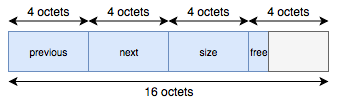
\includegraphics[scale=0.7]{images/heap_header.png}
  \caption{Entête d'un bloc de mémoire dans le tas}
  \label{heap_header}
\end{figure}

Le tas ainsi construit, avec chaque entête lié à ses voisins par des pointeurs,
permet de rechercher aisément un bloc libre. Un nouvel entête est créé quand le
dernier bloc de la liste chaînée est alloué. Un algorithme a aussi été implémenter
pour la gestion de mémoire libérée. Si un bloc est libéré au milieu de blocs
alloués ce blocs est simplement marqué comme libre (en utilisant le booléen \textit{free}
de l'entête). Si deux blocs libres sont contiguës, ils sont fusionnés pour n'en
former qu'un seul. Dans le \textit{kernel}, la fonction pour l'allocation est
\mintinline{rust}{kmalloc} et la fonction pour la libération est \mintinline{rust}{kfree}.
La fonction \mintinline{rust}{kmalloc} va allouer de nouvelles pages et tables
de pages automatiquement s'il y a besoin (comme le montre la figure \ref{kmalloc}).
De la même manière, la fonction \mintinline{rust}{kfree} va libérer les pages et
les tables de pages automatiquement. Ces deux fonctions permettent donc beaucoup
d'abstraction au niveau de la pagination mais aussi de l'allocation car l'utilisation
des entêtes est complètement transparent. La fonction \mintinline{rust}{kmalloc}
va simplement renvoyer une adresse sur 32 bits et \mintinline{rust}{kfree} prend
comme argument cette adresse pour libérer la mémoire.

\begin{figure}[!h]
  \centering
  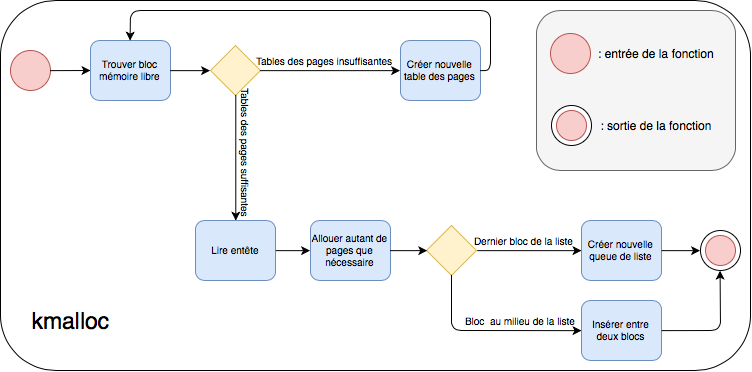
\includegraphics[scale=0.6]{images/kmalloc.png}
  \caption{Algorithme utilisé pour l'allocation dynamique dans le \textit{kernel}}
  \label{kmalloc}
\end{figure}

Voyons maintenant un exemple d'allocation et de libération mémoire utilisant les
deux algorithmes décrits ci-dessus. Dans cet exemple, nous allons allouer plusieurs
blocs mémoire puis les libérer afin de voir plus en détail le comportement
de ces fonctions. Nous allons supposé que la fin du \textit{kernel} se situe
à l'adresse 0x3FC000 et que la fin de la \acrshort{ram} se situe à l'adresse
0x1000000. A l'initialisation du \textit{kernel}, un premier entête est créé au
début de la zone d'allocation dynamique. Ce premier entête est donc situé à
l'adresse 0x3FC000 et a pour taille 0x1000000 $-$ 0x3FC000 $=$ 0xC04000. C'est cette
information qui permet de trouver la premier entrée de la liste et par la suite
de la parcourir.

\begin{figure}[!h]
  \centering
  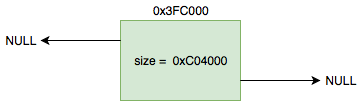
\includegraphics[scale=0.7]{images/alloc0.png}
  \caption{Etat initial de la chaîne d'entêtes}
  \label{alloc0}
\end{figure}

Si le \textit{kernel} a besoin d'allouer une nouvelle page maintenant, la fonction
\ref{kmalloc} va être appelée qui va parcourir les blocs libre. Dans ce cas précis,
l'intégralité du tas est disponible donc la fonction va simplement créer un nouveau
bloc. Dans la figure \ref{alloc1}, les blocs libre sont en vert et les blocs alloués
sont en rouge. A noter que que les blocs aloués sont alignés avec la taille d'une
page (4096Ko ou 0x1000 en hexadécimal). Etant donné qu'il faut compté l'entête
de 16 octets, il faudra toujours allouer une page de plus.

\begin{figure}[!h]
  \centering
  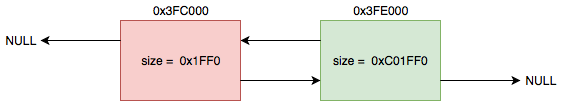
\includegraphics[scale=0.6]{images/alloc1.png}
  \caption{Allocation d'une page}
  \label{alloc1}
\end{figure}

Si le \textit{kernel} a de nouveau besoin d'une page, on va se retrouver dans la
situation où il n'y a plus assez de place dans la table des pages. Pour rappel,
une table des pages a une taille de 4Mo (0x400000 en hexadécimal). Comme expliqué
avec la figure \ref{kmalloc}, la fonction d'allocation va se charge toute seule
de créer une nouvelle table des pages et de l'ajouter au répertoire de pages.
La page demandée par le \textit{kernel} sera ensuite allouée. On obtient donc
la liste de la figure \ref{alloc2}, avec deux blocs alloués au lieu d'un seul.
Le bloc à l'adresse 0x3FE000 contient alors la table des pages sur laquelle pointe
la deuxième entrée du répertoire des pages. La page demandée par le \textit{kernel}
sera finalement à l'adresse 0x400000.

\begin{figure}[!h]
  \centering
  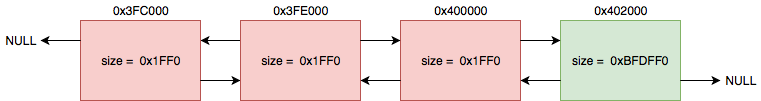
\includegraphics[scale=0.6]{images/alloc2.png}
  \caption{Allocation d'une page et d'une table des pages}
  \label{alloc2}
\end{figure}

Libérer la page à l'adresse 0x400000 aura pour conséquence directe de libérer aussi
la table des pages nouvellement créée (la fonction \mintinline{rust}{kfree} libère
automatiquement les tables des pages vides). On se retrouverait alors avec le même
schéma que dans la figure \ref{alloc1} car les blocs aux adresses 0x3FE000 et
0x400000 seraient fusionnés au reste de la mémoire libre.

\newpage
%%%%%%%%%%%%%%%%%%%%%%%%%%%%%%%%%%%%%%%%%%%%%%%%%%%%%%%%%%%%%%%%%%
%%%%%%%%%%%%%%%%%%%%%%%%%%%%%%%%%%%%%%%%%%%%%%%%%%%%%%%%%%%%%%%%%%

\section{Périphériques}
%%%%%%%%%%%%%%%%%%%%%%%%%%%%%%%%%%%%%%%%%%%%%%%%%%%%%%%%%%%%%%%%%%
%%%%%%%%%%%%%%%%%%%%%%%%%%%%%%%%%%%%%%%%%%%%%%%%%%%%%%%%%%%%%%%%%%

\subsection{Ports}
Un processeur \acrshort{IA-32} a la possibilité de transférer des données en utilisant
les ports d'entrée/sortie. Ces ports sont utilisés par le processeurs pour communiquer
avec des périphériques. Il peuvent être utilisés pour envoyer et recevoir des données
(par exemple un \textit{timer} va utiliser les ports d'entrée/sortie pour envoyer
son état). Les ports peuvent aussi être utilisés pour contrôler un péripéhrique
à partir de registres de contrôle (par exemple avec un controlleur de disque).\cite{ref64}
Etant donné que nous ne sommes pas sur du vrai \textit{hardware}, QEMU va se charger
d'émuler les différents périphériques utilisés par un processeur Intel 32-bits. \\

Les ports d'entrées/sorties sur architecture x86 se situent dans un espace d'adresses
séparé de la mémoire physique. Cet espace permet d'adresser 64000 (soit $2^{16}$)
ports de 8 bits. Les ports sont donc adressés sur 16 bits mais  il n'est pas possible
d'écrire dans un \acrshort{pio} de la même manière que l'on écrirait dans la mémoire
(avec une instruction  \mintinline{text}{MOV}) car nous sommes dans deux
espaces d'adresses différents. Ainsi, le \acrshort{cpu} utilise des instructions speciales
pour accéder aux \acrshort{pio}. Ces instructions sont les instructions
\mintinline{text}{IN} et \mintinline{text}{OUT}. \mintinline{text}{IN} permet de lire
tandis que \mintinline{text}{OUT} permet d'écrire. A noter que l'adresse du port
doit toujours être spécifiée dans le registre \mintinline{text}{dx} et la lecture
et l'écriture se font toujours avec les registres \mintinline{text}{ax/al}.\cite{ref42} \\

\begin{multicols}{2}
    [
    Exemple de lecture et d'écriture dans un port d'entrée/sortie :
    ]
    Ecrire 4 dans le port 0x2A :
    \begin{minted}[fontsize=\footnotesize,tabsize=4]{text}
        mov dx, 0x2A
        mov al, 4
        out dx, al
    \end{minted}
    \columnbreak
    Lire un octet depuis le port 0x2A :
    \begin{minted}[fontsize=\footnotesize,tabsize=4]{text}
        mov dx, 0x2A
        in  byte al, dx
    \end{minted}
\end{multicols}

Il existe une autre méthode pour écrire dans les ports utilisant le même bus d'adresse
pour la mémoire physique et pour les périphériques. Cette méthode consiste à
\textit{mapper} les ports d'entrées/sorties dans la mémoire physique (\acrshort{mmio}).
En écrivant dans la zone reservée aux ports, on écrirait alors directement dans
les ports et pas dans la mémoire physique. Le \textit{kernel} développé utilise
la première méthode (\acrshort{pio}).

%%%%%%%%%%%%%%%%%%%%%%%%%%%%%%%%%%%%%%%%%%%%%%%%%%%%%%%%%%%%%%%%%%
%%%%%%%%%%%%%%%%%%%%%%%%%%%%%%%%%%%%%%%%%%%%%%%%%%%%%%%%%%%%%%%%%%

\subsection{Interruptions et Exceptions}
\subsubsection{Principe général}
Les interruptions et les exceptions sont des évenements qui indiquent que l'attention
du processeur est demandée quelque part soit dans le code, soit par un périphérique.
Il existe deux types d'interruptions, les interruptions logicielles et les interruptions
matérielles. Les exceptions sont générées par le processeur mais diffèrent des
interruptions logicielles. Une interruption peut arriver à n'importe quel moment
en réponse au signal d'un périphérique ou bien si le processeur le demande
avec l'instruction \mintinline{text}{INT} (interruption logicielle). Une exception
est levée lorsque le processeur détecte une erreur à l'exécution d'une instruction
(par exemple une division par 0). Quand une interruption ou une exception
a lieu, une routine logicielle est appelée (\acrshort{isr}). Les processeurs \acrshort{IA-32}
supportent jusqu'à 256 interruptions dont les 32 premières sont reservées aux exceptions
processeur (voir figure \ref{table_int_exc}).\cite{ref42,ref66} \\

\begin{figure}[!h]
  \centering
  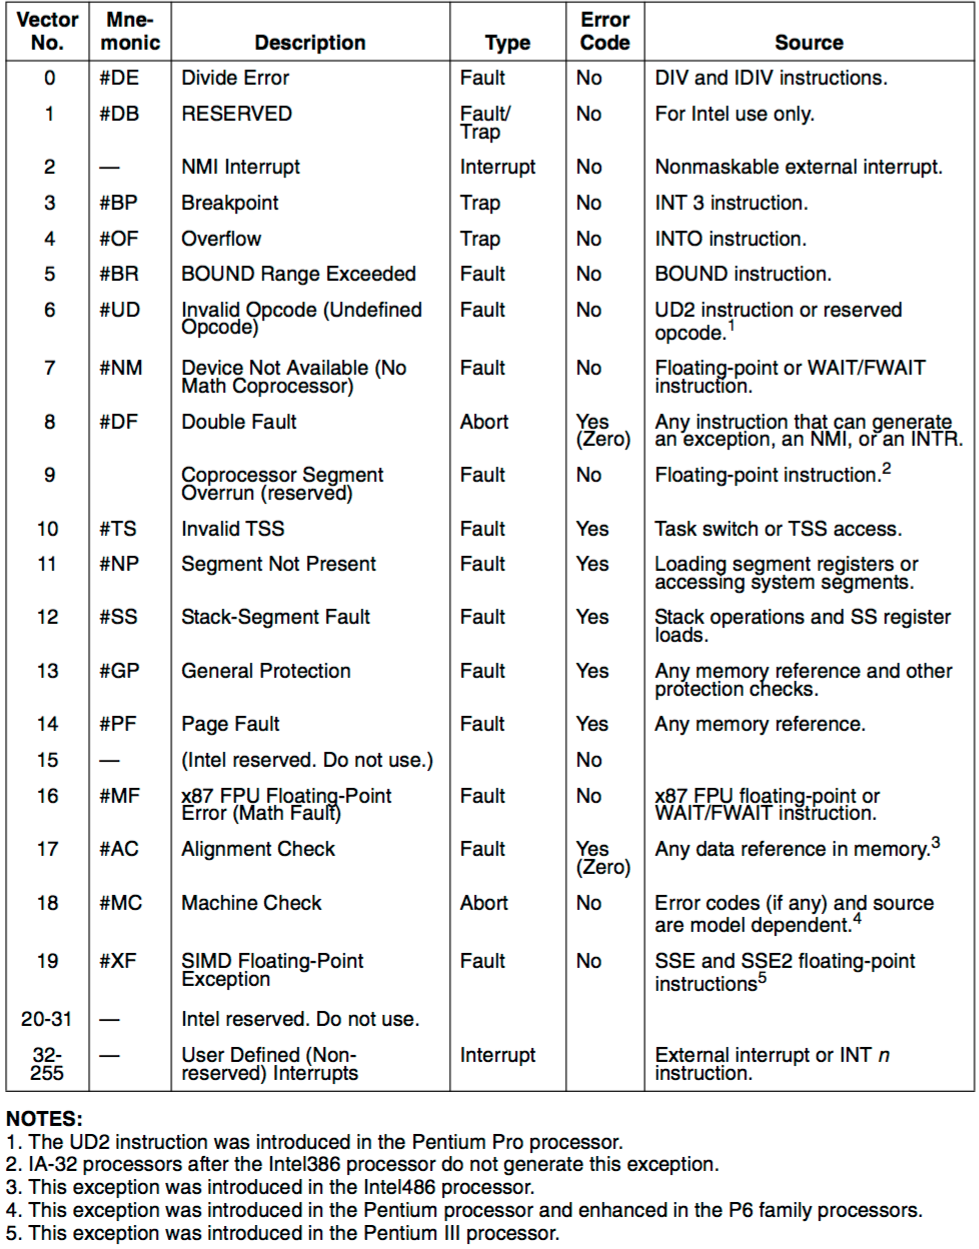
\includegraphics[scale=0.39]{images/table_int_exc.png}
  \caption{Table des interruptions et exceptions sur \acrshort{IA-32}}
  \label{table_int_exc}
\end{figure}

Comme vu précedemment, une interruption logicielle peut être exécutée par le
processeur avec l'instruction \mintinline{text}{INT}. L'instruction \mintinline{text}{INT}
suivie du numéro d'interruption sur 8 bits déclenchera l'interruption en question.
Par exemple, l'instruction \mintinline{text}{INT 0x30} déclenchera l'interruption
48. Au moment de l'appel à l'instruction \mintinline{text}{INT}, le pointeur
d'instruction va sauter à l'adresse du code contennant la routine d'interruption
correspondant au numéro d'interruption logicielle specifiée. C'est la table des
descripteurs d'interruption (\acrshort{idt}) qui permet de définir l'adresse du
code à exécuter pour chaque numéro d'interruption (que ce soit une interruption
logicielle, matérielle ou une exception). A noter aussi que les interruptions
logicielles sont synchrone étant donné qu'elles sont exécutées par le processeur,
contrairement aux interruptions matérielles qui sont asynchrones (exécutées par
les périphériques, elle peuvent arriver à n'importe quel moment). \\

Nous avons vu que les interruptions matérielles étaient générées par le \textit{hardware}.
Il existe deux types d'interruptions matérielles, les \acrshort{nmi} (\textit{Non Maskable
Interrupt}) et les \acrshort{irq} (Interrupt Request). Une \acrshort{nmi} indique
qu'un problème est survenu au niveau matériel (mémoire défectueuse, erreur de bus, ...).
Comme son nom l'indique, une \acrshort{nmi} ne peut pas être ignorée (ou masquée),
l'interruption doit donc dans tous les cas être servie. Le but ici est d'arrêter
le processeur afin d'éviter toute perte de données.\cite{ref42} Une \acrshort{irq}
quant à elle peut être masquée. L'instruction \mintinline{text}{CLI} permet de masquer
les interruptions et l'instruction \mintinline{text}{STI} permet de les démasquer.
En général, un périphérique génère une \acrshort{irq} lorsque des données sont
prêtes à être lues, qu'une commande est terminée ou qu'un évenement particulier
a lieu (par exemple la pression d'une touche du clavier ou l'écriture de données
sur le disque). Quand une interruption est générée, l'\acrshort{isr} correspondant
à l'\acrshort{irq} doit être appelée. C'est là qu'entre en jeu le controlleur
d'interruption (\acrshort{pic}). Le \acrshort{pic} va faire correspondre une
\acrshort{irq} à un numéro d'interruption (voir figure \ref{irqs}). A la manière des
interruptions logicielles l'\acrshort{idt} va être utilisée pour appeler la bonne
routine d'interruption. Le \acrshort{pic} permet donc de faire le lien entre le
matériel et le logiciel. \\

\begin{figure}[!h]
  \centering
  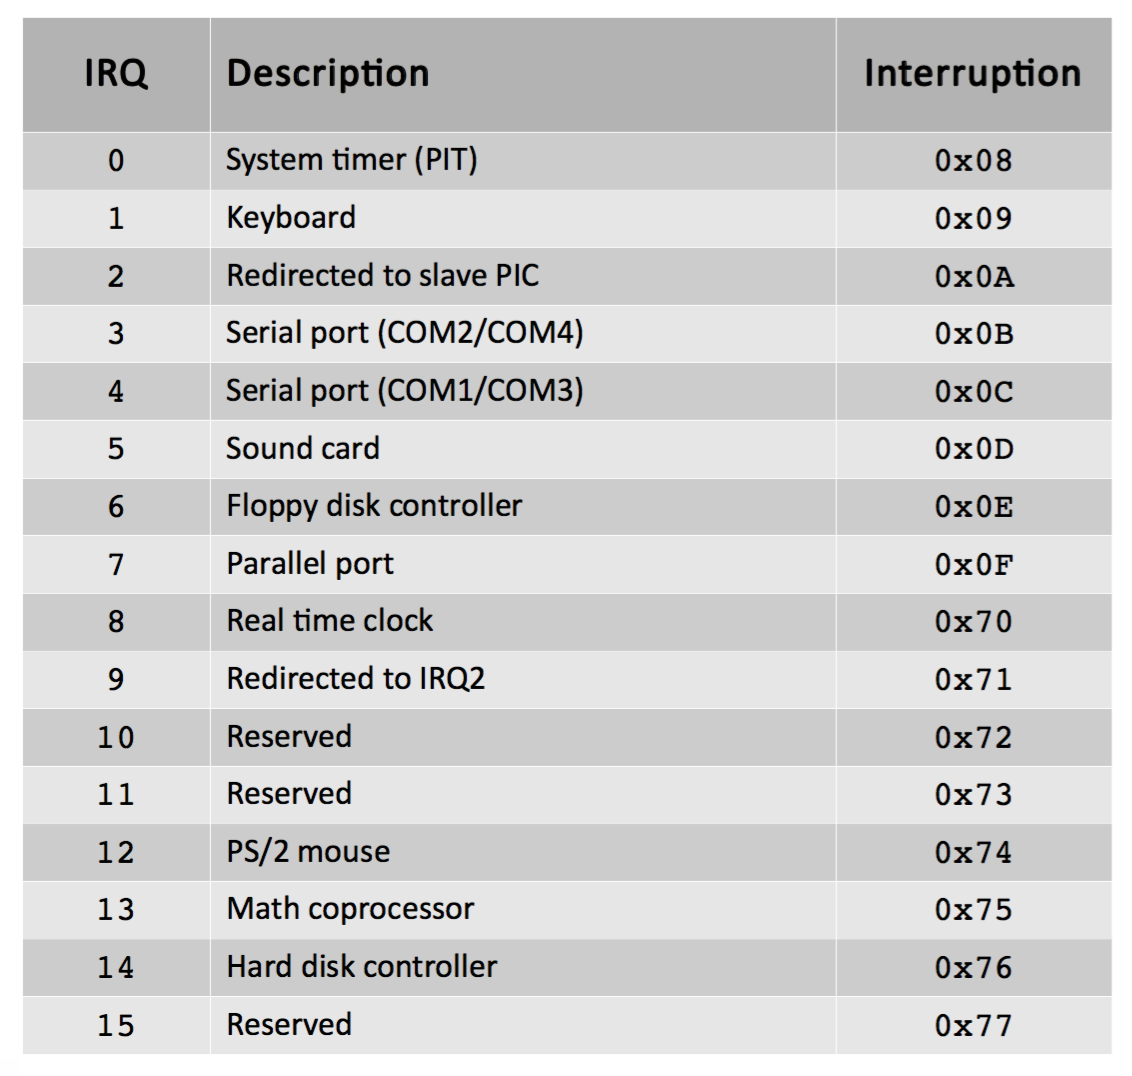
\includegraphics[scale=0.5]{images/irqs.png}
  \caption{Table de correspondance des \acrshort{irq}s}
  \label{irqs}
\end{figure}

En comparant la figure \ref{table_int_exc} avec la figure \ref{irqs}, on constate
que certaines \acrshort{irq}s partagent le même numéro d'interruption que des
exceptions. L'interruption du \textit{timer} par exemple a le même numéro d'interruption
que l'exception \textit{Double Fault} (0x8). Si on laisse le \textit{mapping} par
défaut, une interruption du \textit{timer} va déclencher une \textit{Double Fault}
ce qui n'est pas souhaitable. Il a donc été nécessaire de changer cette table
de correspondance. Les \acrshort{irq}s 0 à 7 ont été associées aux interruptions
32 à 39 et les \acrshort{irq}s 8 à 15 ont été associées aux interruptions 40 à 47.
Ce changement de \textit{mapping} peut se faire assez simplement en assembleur en
utilisant les ports des deux \acrshort{pic}s utilisés par les \acrshort{irq}s.
Un code d'exemple est donné sur le site OSDev.\cite{ref22}

%%%%%%%%%%%%%%%%%%%%%%%%%%%%%%%%%%%%%%%%%%%%%%%%%%%%%%%%%%%%%%%%%%

\subsubsection{\acrshort{idt}}
La table des descripteurs d'interruption (ou \acrshort{idt}) est similaire à la
\acrshort{gdt} (la table des descripteurs globaux). Elle est aussi composée de
descripteurs de 64-bits permettant chacun de référencer une interruption. Un
descripteur est composé d'un offset indiquant l'adresse de l'\acrshort{isr} (la
routine d'interruption), un selecteur de segment indiquant le segment où se trouve
le code de l'\acrshort{isr} et un niveau de privilège indiquant le niveau de privilège
requis pour exécuter l'\acrshort{isr}. Dans le cas d'un adressage de type \textit{FLAT}
comme celui utilisé, le selecteur de segment sera forcément le selecteur de segment
de code. Il existe aussi plusieurs types de descripteurs d'interruptions\cite{ref66}
décrits dans la figure \ref{idt_entry}. Dans le cas de notre \textit{kernel} seulement
deux types ont été utilisés, le type \textit{Interrupt Gate} et le type \textit{Trap Gate}.
La différence entre un \textit{Interrupt Gate} et un \textit{Trap Gate} est uniquement
le comportement du \acrshort{cpu} lors de l'exécution de l'\acrshort{isr}\cite{ref42}.
Dans le cas du \textit{Interrupt Gate}, le \acrshort{cpu} masquera les interruptions
lors de l'exécution de l'\acrshort{isr} alors que dans un \textit{Trap Gate} ce
ne sera pas le cas. \\

\begin{figure}[!h]
  \centering
  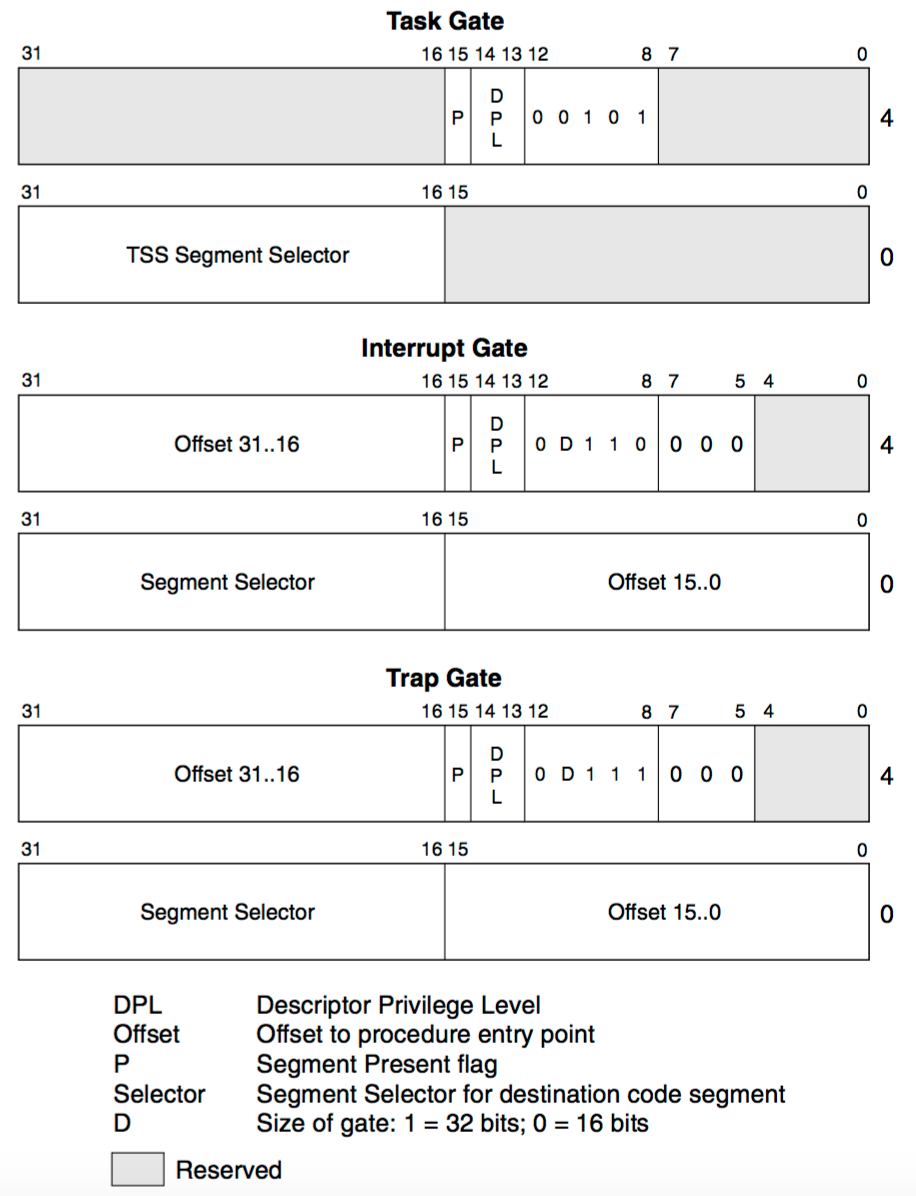
\includegraphics[scale=0.75]{images/idt_entry.png}
  \caption{Différents types de descripteur d'interruption}
  \label{idt_entry}
\end{figure}

Comme pour la \acrshort{gdt}, l'\acrshort{idt} est stockée en \acrshort{ram}
et doit donc être initialisée et gérée par l'\acrshort{os}. De la même manière
que l'instruction \mintinline{text}{LGDT} permet de charger la \acrshort{gdt},
l'instruction \mintinline{text}{LIDT} permet de charger l'\acrshort{idt} dans le
registre IDTR. Pour se faire il faut donner comme argument à l'instruction 
\mintinline{text}{LIDT} l'adresse du descripteur d'\acrshort{idt} sur 48 bits.
Ce descripteur est composé de l'adresse de l'\acrshort{idt} sur 32 bits et de sa
limite (sa taille en bytes - 1) sur 16 bits. Une fois la table des descripteurs
d'interruption chargée avec l'instruction \mintinline{text}{LIDT}, les interruptions
peuvent être activées en utilisant l'instruction \mintinline{text}{STI}. La figure
\ref{idtr} permet de résumer la relation entre le registre IDTR et l'\acrshort{idt}.

\begin{figure}[!h]
  \centering
  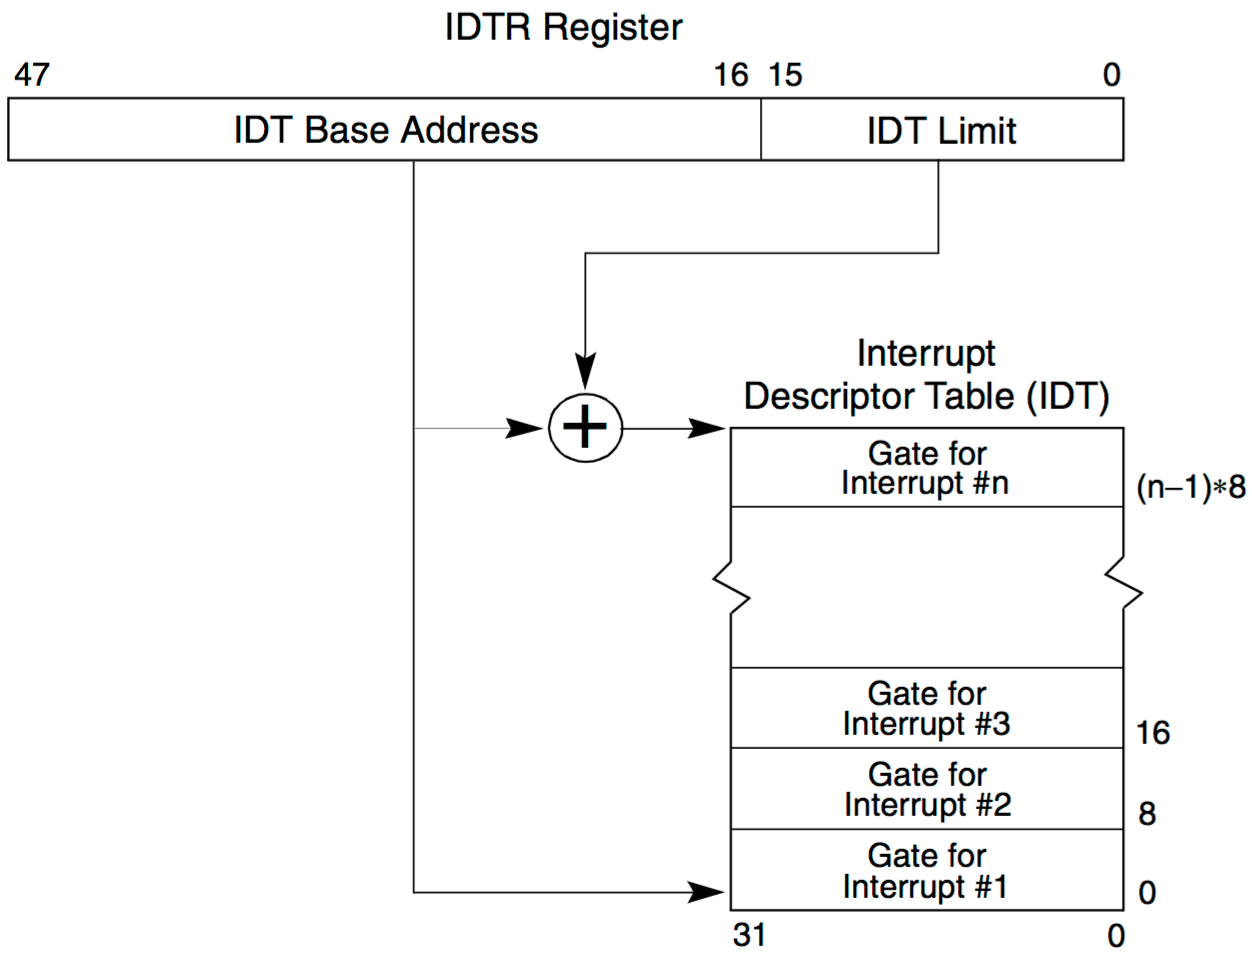
\includegraphics[scale=0.6]{images/idtr.png}
  \caption{Relation entre le registre IDTR et l'\acrshort{idt}}
  \label{idtr}
\end{figure}

Dans le \textit{kernel} développé, l'\acrshort{idt} est une structure statique
en mémoire. Une fonction assembleur est donc appelée afin de charger cette
structure dans le registre IDTR. En plus du chargement de l'\acrshort{idt}, une
partie des routines d'interruptions est faite en assembleur. En effet, il a été
nécéssaire de passer par du code bas niveau car avant de rentrer dans une
routine d'interruption, il faut sauvegarder le contexte. Il est obligatoire
de sauvegarder le contexte car, comme déjà dit plus haut, une interruption
peut avoir lieu à n'importe quel moment. La partie bas niveau de la routine
d'interruption s'occupe donc de sauvegarder le contexte puis d'appeler un
gestionnaire d'interruption haut niveau en rust. Ce gestionnaire prend comme argument
le numéro d'interruption et appelle la routine d'interruption liée à cette interruption.
Par exemple, la routine d'interruption du \textit{timer} va simplement incrémenter
un compteur. Lorsque une exception est levée le même mécanisme est employé sauf
qu'ici le \textit{kernel} va afficher un message d'erreur en fonction du numéro
de l'exception.

%%%%%%%%%%%%%%%%%%%%%%%%%%%%%%%%%%%%%%%%%%%%%%%%%%%%%%%%%%%%%%%%%%
%%%%%%%%%%%%%%%%%%%%%%%%%%%%%%%%%%%%%%%%%%%%%%%%%%%%%%%%%%%%%%%%%%

\subsection{\acrshort{vga}}
Un \acrshort{pc} possède généralement une carte graphique permettant de gérer
l'affichage. Une grande majorité des carte graphiques, même modernes sont compatibles
avec le standard d'affichage \acrshort{vga}. Dans notre cas, nous utilisons un
émulateur (QEMU) qui va émuler l'affichage \acrshort{vga}. Pour écrire sur l'écran
il faut écrire dans la mémoire vidéo (\acrshort{vram}) qui commence à l'adresse
0xA0000 et finit à l'adresse 0xBFFFF. Différents modes d'écriture existent pour
l'affichage mais nous allons nous concentrer sur un seul en particulier. \\

Le mode texte \acrshort{vga} a été utilisé pour l'affichage dans l'\acrshort{os}
développé. En mode texte, l'écran est divisé en caractères plutôt qu'en pixels ce
qui permet d'afficher simplement et rapidement quelque chose sur l'écran. La mémoire
vidéo reservée au mode texte commence à l'adresse 0xB8000 et a une taille de
$80 \times 25$ caractères. Un caractère est représenté par 2 octets (16 bits) ce
qui fait une taille de 4000 octets ($80 \times 25 \times 2$). L'octet de poids
faible d'un caractère représente la valeur ASCII de ce caractère et l'octet de poids
fort représente l'attribut qui contient lui même la couleur du caractère et la
couleur du fond (voir figure \ref{vga_char}) \cite{ref42}. La couleur en mode texte
est donc codée sur 4 bits ce qui fait 16 couleurs différentes. Ces 16 couleurs sont
décrites dans la figure \ref{colors} \cite{ref19}. \\

\begin{figure}[!h]
  \centering
  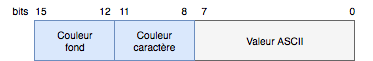
\includegraphics[scale=0.8]{images/vga_char.png}
  \caption{Structure d'un caractère en mode texte \acrshort{vga}}
  \label{vga_char}
\end{figure}

\begin{figure}[!h]
  \centering
  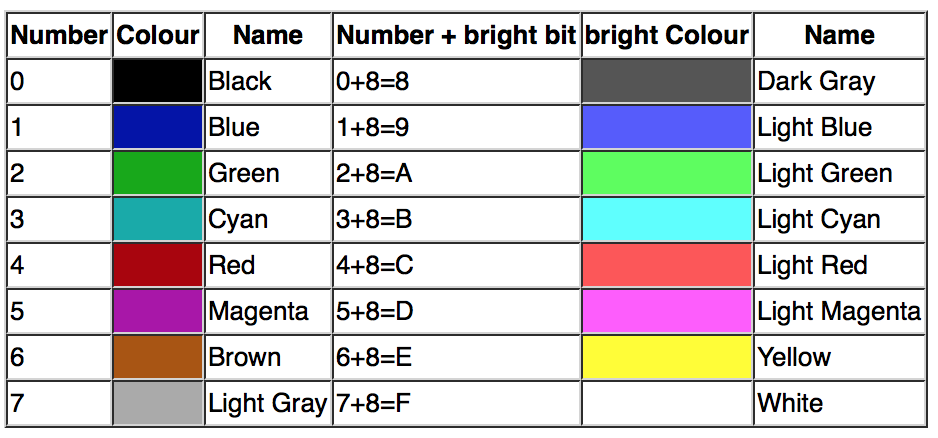
\includegraphics[scale=0.7]{images/colors.png}
  \caption{Couleurs disponibles en mode texte \acrshort{vga}}
  \label{colors}
\end{figure}

Le mode texte \acrshort{vga} permet aussi d'afficher un curseur. Le curseur ne
se déplace pas automatiquement quand un caractère est écrit à l'écran, c'est
simplement une zone de l'écran mise en évidence par un clignotement et dont
la taille, la position et la visibilité peuvent être modifiés \cite{ref23}. L'accès
au curseur se fait en utilisant les registres du \acrshort{crtc} (\textit{Cathode Ray
Tube Controller}). Les registres du \acrshort{crtc} peuvent être accédés avec la
paire registre d'adresse et registre de données. Ces regsitres se trouvent respectivement
aux ports 0x3D4 et 0x3D5. L'écriture dans un registre du \acrshort{crtc} se fait
donc en deux temps. Tout d'abord, l'adresse du registre doit être specifiée
en écrivant dans le port 0x3D4 puis la donnée doit être écrite dans le port 0x3D5
\cite{ref42}.

%%%%%%%%%%%%%%%%%%%%%%%%%%%%%%%%%%%%%%%%%%%%%%%%%%%%%%%%%%%%%%%%%%
%%%%%%%%%%%%%%%%%%%%%%%%%%%%%%%%%%%%%%%%%%%%%%%%%%%%%%%%%%%%%%%%%%

\subsection{\textit{Timer}}

%%%%%%%%%%%%%%%%%%%%%%%%%%%%%%%%%%%%%%%%%%%%%%%%%%%%%%%%%%%%%%%%%%
%%%%%%%%%%%%%%%%%%%%%%%%%%%%%%%%%%%%%%%%%%%%%%%%%%%%%%%%%%%%%%%%%%

\subsection{Clavier}

\newpage
%%%%%%%%%%%%%%%%%%%%%%%%%%%%%%%%%%%%%%%%%%%%%%%%%%%%%%%%%%%%%%%%%%
%%%%%%%%%%%%%%%%%%%%%%%%%%%%%%%%%%%%%%%%%%%%%%%%%%%%%%%%%%%%%%%%%%

\section{Système de fichiers}
%%%%%%%%%%%%%%%%%%%%%%%%%%%%%%%%%%%%%%%%%%%%%%%%%%%%%%%%%%%%%%%%%%
%%%%%%%%%%%%%%%%%%%%%%%%%%%%%%%%%%%%%%%%%%%%%%%%%%%%%%%%%%%%%%%%%%

\subsection{Introduction}

%%%%%%%%%%%%%%%%%%%%%%%%%%%%%%%%%%%%%%%%%%%%%%%%%%%%%%%%%%%%%%%%%%
%%%%%%%%%%%%%%%%%%%%%%%%%%%%%%%%%%%%%%%%%%%%%%%%%%%%%%%%%%%%%%%%%%

\subsection{Structure}


\newpage
%%%%%%%%%%%%%%%%%%%%%%%%%%%%%%%%%%%%%%%%%%%%%%%%%%%%%%%%%%%%%%%%%%
%%%%%%%%%%%%%%%%%%%%%%%%%%%%%%%%%%%%%%%%%%%%%%%%%%%%%%%%%%%%%%%%%%

\section{Tâches utilisateur}

\newpage
%%%%%%%%%%%%%%%%%%%%%%%%%%%%%%%%%%%%%%%%%%%%%%%%%%%%%%%%%%%%%%%%%%
%%%%%%%%%%%%%%%%%%%%%%%%%%%%%%%%%%%%%%%%%%%%%%%%%%%%%%%%%%%%%%%%%%

\section{Résultats}

\newpage
%%%%%%%%%%%%%%%%%%%%%%%%%%%%%%%%%%%%%%%%%%%%%%%%%%%%%%%%%%%%%%%%%%
%%%%%%%%%%%%%%%%%%%%%%%%%%%%%%%%%%%%%%%%%%%%%%%%%%%%%%%%%%%%%%%%%%

\section{Discussions}
\subsection{Problèmes rencontrés}

%%%%%%%%%%%%%%%%%%%%%%%%%%%%%%%%%%%%%%%%%%%%%%%%%%%%%%%%%%%%%%%%%%

\subsection{Améliorations possibles}

\newpage
%%%%%%%%%%%%%%%%%%%%%%%%%%%%%%%%%%%%%%%%%%%%%%%%%%%%%%%%%%%%%%%%%%
%%%%%%%%%%%%%%%%%%%%%%%%%%%%%%%%%%%%%%%%%%%%%%%%%%%%%%%%%%%%%%%%%%

\section{Conclusion}

\newpage
%%%%%%%%%%%%%%%%%%%%%%%%%%%%%%%%%%%%%%%%%%%%%%%%%%%%%%%%%%%%%%%%%%
%%%%%%%%%%%%%%%%%%%%%%%%%%%%%%%%%%%%%%%%%%%%%%%%%%%%%%%%%%%%%%%%%%

\section{Références}
\nocite{*}
\bibliographystyle{unsrt}
\bibliography{biblio}

\end{document}
